\pdfoutput=1
\pdfcompresslevel=9
\pdfinfo
{
    /Author ()
    /Title ()
    /Subject ()
    /Keywords ()
}

\batchmode
\nonstopmode

%\newcommand*{\memfontfamily}{pnc}
%\newcommand*{\memfontpack}{newcent}
\documentclass[a4paper,onecolumn,oneside,12pt]{memoir}
% Wydruk do archiwum
%\documentclass[a4paper,onecolumn,twoside,10pt]{memoir} 
%\renewcommand{\normalsize}{\fontsize{8pt}{10pt}\selectfont}
\usepackage[utf8]{inputenc}
\usepackage[T1]{fontenc}
\usepackage{setspace}
\usepackage{tabularx}
\usepackage{color,calc}
\usepackage[]{algorithm2e}
%\usepackage{soul} % pakiet z komendami do podkreślania tekstu
\usepackage{times} % pakiet zmieniający czcionki na times 

%\usepackage{longtable}
%\usepackage{ltxtable}
%\usepackage{tabulary}

\usepackage{indentfirst}
\usepackage{multicol}
\usepackage{listings}
\lstset{basicstyle=\footnotesize\ttfamily,breaklines=true}

%%%%%% Ustawienia odpowiedzialne za sposób łamania dokumentu
%\hyphenpenalty=10000		% nie dziel wyrazów zbyt często
\clubpenalty=10000      %kara za sierotki
\widowpenalty=10000  % nie pozostawiaj wdów
\brokenpenalty=10000		% nie dziel wyrazów między stronami
\exhyphenpenalty=999999		% nie dziel słów z myślnikiem
\righthyphenmin=3			% dziel minimum 3 litery

%\tolerance=4500
%\pretolerance=250
%\hfuzz=1.5pt
%\hbadness=1450

%ustawienia rozmiarów: tekstu, stopki, marginesów 
\setlength{\textwidth}{\paperwidth}
\addtolength{\textwidth}{-5cm}
\setlength{\textheight}{\paperheight}
\addtolength{\textheight}{-5cm}
\setlength{\oddsidemargin}{-0.04cm} % domyślnie jest 1 cal = 2.54 cm, stąd -0.04 da margines 2.5cm
\setlength{\evensidemargin}{-0.04cm} % domyślnie jest 1 cal = 2.54 cm, stąd -0.04 da margines 2.5cm
\topmargin -1.25cm 
\footskip 1.4cm 

\linespread{1}
%\linespread{1.3}

\usepackage{ifpdf}
%\newif\ifpdf \ifx\pdfoutput\undefined
%\pdffalse % we are not running PDFLaTeX
%\else
%\pdfoutput=1 % we are running PDFLaTeX
%\pdftrue \fi
\ifpdf
\usepackage[pdftex]{graphicx,hyperref}
\DeclareGraphicsExtensions{.pdf,.jpg,.mps,.png}
\pdfcompresslevel=9
\else
\usepackage{graphicx}
\DeclareGraphicsExtensions{.eps,.ps,.jpg,.mps,.png}
\fi
\sloppy

%\graphicspath{{rys01/}{rys02/}}
%\usepackage{rotating}

\renewcommand{\topfraction}{1.0}
\renewcommand{\bottomfraction}{1.0}
\renewcommand{\textfraction}{0.0}
\renewcommand{\floatpagefraction}{0.35}

%%%%%%%%%%%%%%%%%%%%%%%%%%%%%%%%%%%%%%%
%                  Definicja strony tytułowej 
%%%%%%%%%%%%%%%%%%%%%%%%%%%%%%%%%%%%%%%
\makeatletter
%Uczelnia
\newcommand\uczelnia[1]{\renewcommand\@uczelnia{#1}}
\newcommand\@uczelnia{}
%Wydział
\newcommand\wydzial[1]{\renewcommand\@wydzial{#1}}
\newcommand\@wydzial{}
%Kierunek
\newcommand\kierunek[1]{\renewcommand\@kierunek{#1}}
\newcommand\@kierunek{}
%Specjalność
\newcommand\specjalnosc[1]{\renewcommand\@specjalnosc{#1}}
\newcommand\@specjalnosc{}
%Tytuł po angielsku
\newcommand\titleEN[1]{\renewcommand\@titleEN{#1}}
\newcommand\@titleEN{}
%Tytuł krótki
\newcommand\titleShort[1]{\renewcommand\@titleShort{#1}}
\newcommand\@titleShort{}
%Promotor
\newcommand\promotor[1]{\renewcommand\@promotor{#1}}
\newcommand\@promotor{}

\def\maketitle{%
  \null
  \pagestyle{empty}%i
	{\centering\vspace{-1cm}
		{\fontsize{22pt}{24pt}\selectfont \@uczelnia}\\[0.4cm]
		{\fontsize{22pt}{24pt}\selectfont \@wydzial }\\[0.5cm]
		\hrule \vspace*{0.7cm}
	}
{\flushleft\fontsize{14pt}{16pt}\selectfont%
\begin{tabular}{ll}
KIERUNEK: & \@kierunek\\
SPECJALNOŚĆ: & \@specjalnosc\\
\end{tabular}\\[1.3cm]
}
{\centering
\vskip 1cm
{\fontsize{24pt}{26pt}\selectfont PRACA DYPLOMOWA}\\[0.5cm]
{\fontsize{24pt}{26pt}\selectfont MAGISTERSKA}\\[2cm]
%{\fontsize{24pt}{26pt}\selectfont PROJEKT INżYNIERSKI}\\[1.5cm]
\vskip 0.8cm
}
%
\begin{tabularx}{\linewidth}{p{6cm}>{\centering\arraybackslash}X}
		&{\fontsize{16pt}{18pt}\selectfont \@title}\\[5mm] 	%UWAGA: tutaj jest miejsce na tytył w języku polskim
		&{\fontsize{16pt}{18pt}\selectfont \@titleEN}\\[10mm] %UWAGA: tutaj jest miejsce na tytył w języku angielskim
\end{tabularx}
\vfill
\begin{tabularx}{\linewidth}{p{6cm}l}
		%UWAGA: tutaj jest miejsce na autora pracy
		&{\fontsize{16pt}{18pt}\selectfont AUTOR:}\\[5mm]
		&{\fontsize{14pt}{16pt}\selectfont \@author}\\[10mm]
		%UWAGA: tutaj jest miejsce na promotora pracy 
		&{\fontsize{16pt}{18pt}\selectfont PROWADZĄCY PRACĘ:}\\[5mm]
		&{\fontsize{14pt}{16pt}\selectfont \@promotor}\\[10mm]
		&{\fontsize{16pt}{18pt}\selectfont OCENA PRACY:}\\[20mm]
	\end{tabularx}
\hrule\vspace*{0.3cm}
{\centering
%{\fontsize{24pt}{26pt}\selectfont PRACA DYPLOMOWA}\\[0.5cm]
%{\fontsize{24pt}{26pt}\selectfont MAGISTERSKA}\\[2cm]
{\fontsize{16pt}{18pt}\selectfont \@date}\\[0cm]
}
\normalfont
 \cleardoublepage
}
\makeatother
%%%%%%%%%%%%%%%%%%%%%%%%%%%%%%%%%%%%%%%
%                  Styl rozdziałów 
%%%%%%%%%%%%%%%%%%%%%%%%%%%%%%%%%%%%%%%
\setcounter{secnumdepth}{3}
\setcounter{tocdepth}{3}
%\definecolor{niceblue}{rgb}{.168,.234,.671}

%\AtBeginDocument{% 
%        \addto\captionspolish{% 
%        \renewcommand{\tablename}{Table}% 
%}%} 

%\AtBeginDocument{% 
%        \addto\captionspolish{% 
%        \renewcommand{\chaptername}{Rozdział}% 
%}} 

%\AtBeginDocument{% 
%        \addto\captionspolish{% 
%        \renewcommand{\figurename}{Image}% 
%}%}
%        \addto\captionspolish{% 
%        \renewcommand{\bibname}{Literature}% 
%}


%%%%%%%%%%%%%%%%%%%%%%%%%%%%%%%%%%%%% nowe itemize
\makeatletter
\renewenvironment{itemize}{
  \begin{list}{  
  \csname labelitem\romannumeral\the\@listdepth\endcsname}{
  \setlength{\leftmargin}{1em}
	\setlength{\topsep}{6pt}%
	\setlength{\partopsep}{0pt}%
	\setlength{\parskip}{0pt}%
	\setlength{\parsep}{0pt}%
	\setlength{\itemsep}{0pt}}
}{
  \end{list}
}

%%%%%%%%%%%%%%%%%%%%%%%%%%%%%%%%%%%%%%%%%%%%%%%%%%%%%%%%%%%%%%%%%% Styl wyliczenia (opis skrótów) 
%%%%%%%%%%%%%%%%%%%%%%%%%%%%%%%%%%%%%%%%%%%%%%%%%%%%%%%%%%%%%%%%%
\newenvironment{Ventry}[1]%
 {\begin{list}{}{\renewcommand{\makelabel}[1]{\textbf{##1}\hfill}%
   \settowidth{\labelwidth}{\textbf{#1}}%
   \setlength{\leftmargin}{3cm}}}%
 {\end{list}}

\addtopsmarks{headings}{%
\nouppercaseheads % added at the beginning
}{%
\createmark{chapter}{both}{shownumber}{}{. \space}
%\createmark{chapter}{left}{shownumber}{}{. \space}
\createmark{section}{right}{shownumber}{}{. \space}
}%use the new settings
\pagestyle{headings}

\newlength\mytemplengtha

\setcounter{secnumdepth}{2}
\setcounter{tocdepth}{2}
\setsecnumdepth{subsection} % activating subsubsec numbering in doc

\makeatletter
\copypagestyle{outer}{headings}
\makeoddhead{outer}{}{}{\slshape\rightmark}
\makeevenhead{outer}{\slshape\leftmark}{}{}
\makeoddfoot{outer}{\@author:~\@titleEN}{}{\thepage}
\makeevenfoot{outer}{\thepage}{}{\@author:~\@titleEN}
\makeheadrule{outer}{\linewidth}{\normalrulethickness}
\makefootrule{outer}{\linewidth}{\normalrulethickness}{6pt}
\makeatother

% fix plain
%\copypagestyle{plain}{outer} % overwrite plain with outer
\makeoddhead{plain}{}{}{} % remove right header
\makeevenhead{plain}{}{}{} % remove left header
\makeevenfoot{plain}{}{}{}
\makeoddfoot{plain}{}{}{}

%\copypagestyle{plain}{outer} % overwrite plain with outer
\makeoddhead{empty}{}{}{} % remove right header
\makeevenhead{empty}{}{}{} % remove left header
\makeevenfoot{empty}{}{}{}
\makeoddfoot{empty}{}{}{}

\pagestyle{outer}

%definicja nagłówków
%\renewcommand{\chaptermark}[1]{\markboth{\ifnum \c@secnumdepth >\z@ \thechapter \ \fi #1}{}} 
%\renewcommand{\chaptermark}[1]{\markboth{\thechapter \ #1}{\thesection \ #1}} 
%\renewcommand{\sectionmark}[1]{\markright{\thesection \ #1}{}} 
%\renewcommand{\chaptermark}[1]{\markboth{\thechapter \MakeUppercase{#1}}{}}

%kropki po numerach sekcji
\makeatletter
\def\@seccntformat#1{\csname the#1\endcsname.\quad}
\def\numberline#1{\hb@xt@\@tempdima{#1\if&#1&\else.\fi\hfil}}
\makeatother

\renewcommand{\chapternumberline}[1]{#1.\quad}
\renewcommand{\cftchapterdotsep}{\cftdotsep}

%\AtBeginDocument{\addtocontents{toc}{\protect\thispagestyle{empty}}}

%\includeonly{wstep,rozdzial01} % jeśli chcemy kompilować tylko fragmenty, to można tu je wpisać
%%%%%%%%%%%%%%%%%%%%%%%%%%%%%%%%%%%%%%%%%
%                  Początek dokumentu 
%%%%%%%%%%%%%%%%%%%%%%%%%%%%%%%%%%%%%%%%%
\begin{document}
\title{Filtracja i segmentacja drukowanych w kolorze obrazów}
\titleShort{Filtracja i segmentacja drukowanych w kolorze obrazów}
\titleEN{Preprocessing and segmentation of color-printed images}
\author{Marcin Wojciechowski}
\uczelnia{POLITECHNIKA WROCŁAWSKA}
\wydzial{WYDZIAŁ ELEKTRONIKI}
\kierunek{INFORMATYKA}
\specjalnosc{Internet Engineering}
\promotor{dr inż. Tomasz Babczyński}
\date{WROCŁAW, 2014}
\maketitle

\pagestyle{outer}
\mbox{}\pdfbookmark[0]{Table of Contents}{spisTresci.1}
\tableofcontents* 
\newpage

\chapter{Introduction}

Beginning of this chapter is focused on a problem background. Next part is a 
full description of the topic and definition of main objectives of this thesis.
Finally there is presented a full structure of this document.

\section{Background}

Nowadays image digitization is a very important topic. It has a lot of practical applications.
For example, it is a very good way to prevent destruction of old photos,
to archive them(to keep them in one place in a digital version) and make it easier to 
send it from one place to another. Unfortunately, basic method of digitization of
images - scanning - has some disadvantages. Due to errors made during a scanning procedure,
input image distortions or quality of a scanning device, resulting digitized images 
have a poor quality. To improve digitization process there are many filtration algorithms,
which task is to solve this problem and to produce an image with better quality.Image digitization 
has another big advantage - there is a possibility to retrieve information from the picture(for 
example: pattern recognition, feature extraction). This feature is handled by segmentation 
algorithms. Although this group is one of the most difficult in image processing, there is a big 
emphasis on a research, due to many advantages of this type of algorithms in practical use.

\section{Problem statement and main objectives}

The main aim of this thesis is to create a filtration and segmentation algorithm, which should
apply to scanned color-printed images. This work is focused on scanned maps. 
Resulting algorithm should be optimized to used it with this type of scanned images. 
Output image should have following properties:

\begin{itemize}
  \item most of distortions should be eliminated;
  \item image should be divided into consistent areas, like forests, lakes, rivers, etc. These areas
        should be marked on the map in a consistent way(it should have the same color);
  \item detected areas should have the same size like in an input image;
  \item small details, like text should be kept and marked in a resulting image.
\end{itemize}

Used fltering algorithms should remove main distortions and all disadvantages of image scanning(like
for example rasters, moro effect). Next, proper segmentation algorithm should be used to detect all
areas in an input map and to divide the map into different, homogenous regions. \\

The final solution - set of algorithms - should be impemented in a chosen programming language.
Created application should be tested on many different scanned maps. Test results should be then
analysed.

\section{Document structure}

This document has been divided into seven chapters and the bibliography at the end.
Below there is a short description of a content for each chapter:

\begin{itemize}
  \item In the first chapter there is a description and the background of the topic, 
        next there are listed main objectives of the work and a problem statement;
  \item In the second chapter there is a theoretical introduction of the problem. There are
        explained all already known filtration and segmentation algorithms used in this work.
        The description consists of the definition, properties and parameters of each method. In the
        second part, there is an analysis of existing research work and solutions of the color
        scanned maps preprocessing problem;
  \item Third chapter focuses on research part of this thesis. There are listed all found problems,
        which should be taken into considerationin the analysis of color scanned maps. In the second
        part of the chapter, there is a full description of filtration and segmentation algorithms
        designed in this work;
  \item Fourth chapter focuses on engineering part of the thesis. There is a description of all
        implementation details of the algorithm;
  \item In the fifth chapter there are presented description of all made tests and their results;
  \item In the last chapter there are conclusions of the thesis.
\end{itemize}

\chapter{Theoretical introduction}

This section contains all needed definitions and concepts needed for a good understanding of the
work. It also covers history and basic usage of digital image processing. The last section is 
focused on actual state of art in the filtration and segmentation of color printed digital images.

\section{Digital image processing}

\subsection{History and usage}

According to \cite{digitalImageProcessing},
digital image processing has a lot of practical applications. It was used first at the beginning of
XX century to send pictures over long distances. Research and development of digital image
processing algorithms  was strongly associated with growth of the computer industry. It was caused
by high computational complexity of this type of algorithms. Further growth began in 1960s. Many 
techniques were developed in organisations like Jet Propulsion Laboratory, Massachusetts Institute
of Technology or Bell Laboratories. It was used in satellite imagery, medical imaging(in 1970s 
computerized tomography was developed), image enhancement, science(for example in geography - 
in research about pollution, archeology - in restoring blured pictures), defence or industry.
Another area of digital image processing focuses on extracting an information from the picture in
a for suitable for computer processing. It is used in a character recognition(OCR), industry(
automatic inspection of production process), military, forensics(recognition of fingerprints) and
weather prediction. \\

Nowadays, with fast computers and signal processors, digital image processing is used widely.
It is mainly caused by its low price and versatility.

\subsection{Basic definitions}

A digital image can be defined as a two dimentional function f(x, y), where x and y denote spatial 
coordinates and f(x, y) is the intensity or gray level of the image at this point. Values of x, y
and f(x, y) should be finite, descrete quantities. Digital image processing refers to processing 
digital images by means of a digital computer. It includes many primitive operations like noise
reduction, contrast enhancement or image sharpening. It also involves more advanced algorithms like
image segmentation(partitioning an image into regions or objects), description of objects,
classification(recognition) of objects and even advanced analysis of an image. Digital image 
processing algorithms take an image as an input. Output depends on a type of the algorithm.
It can be new, processed image or group of attributes taken from an image. Main tasks of digital
image processing are:

\begin{itemize}
  \item Image aquisition;
  \item Image enhancement;
  \item Image restoration;
  \item Wavelets;
  \item Compression;
  \item Feature extraction;
  \item Segmentation;
  \item Recognition.
\end{itemize}

This work focuses mainly on image enhancement and image segmentation. All algorithms used in this 
work are described in next sections.

\section{Image enhancement}

Image enhancement algorithms are one of the simplest and most commonly used group of digital image
processing. Main idea of these algorithms is to improve image quality, bring out obscured details 
or highlight certain features of an image.  The main aim of image enhancement is to process image 
and return an image more suitable, than input for a specific application. Proper image enhancement
algorithms should be chosen for different cases(algorithm solving one problem may be inadequate for
other problems). Image enhancement algorithms can be divided into two groups:

\begin{itemize}
  \item Spatial domain - manipulation of pixels of an image directly;
  \item Frequency domain - modification of Fourier transform of an image.
\end{itemize}

\subsection{Smoothing algorithms}

According to \cite{learningOpenCv}, smoothing is a very simple and frequently used operation. It is
used to reduce noise or camera artifacts. It is also used in an image resolution reduction. In this
work, there are two smoothing algorithms used.

\subsubsection{Gaussian blur}

Gaussian filter is one of the most frequently used filters. According to \cite{learningOpenCv}, 
gaussian blur is done by convolving each point in the input array with a Gaussian kernel and then
summing to produce the output array. Resulting image is a smooth blur. It is used to reduce noise
or image details and as a part of edge detection algorithms. Algorithm has two parameters:

\begin{itemize}
  \item \textit{Radius} - it is a kernel size. The bigger value set, the image is smoother;
  \item \textit{Standard Deviation} in X and Y direction.
\end{itemize}

Example result of a Gaussian Blur filter is shown in a Fig.~\ref{gaussianBlurExample}.

\begin{figure}[ht]
\begin{center}
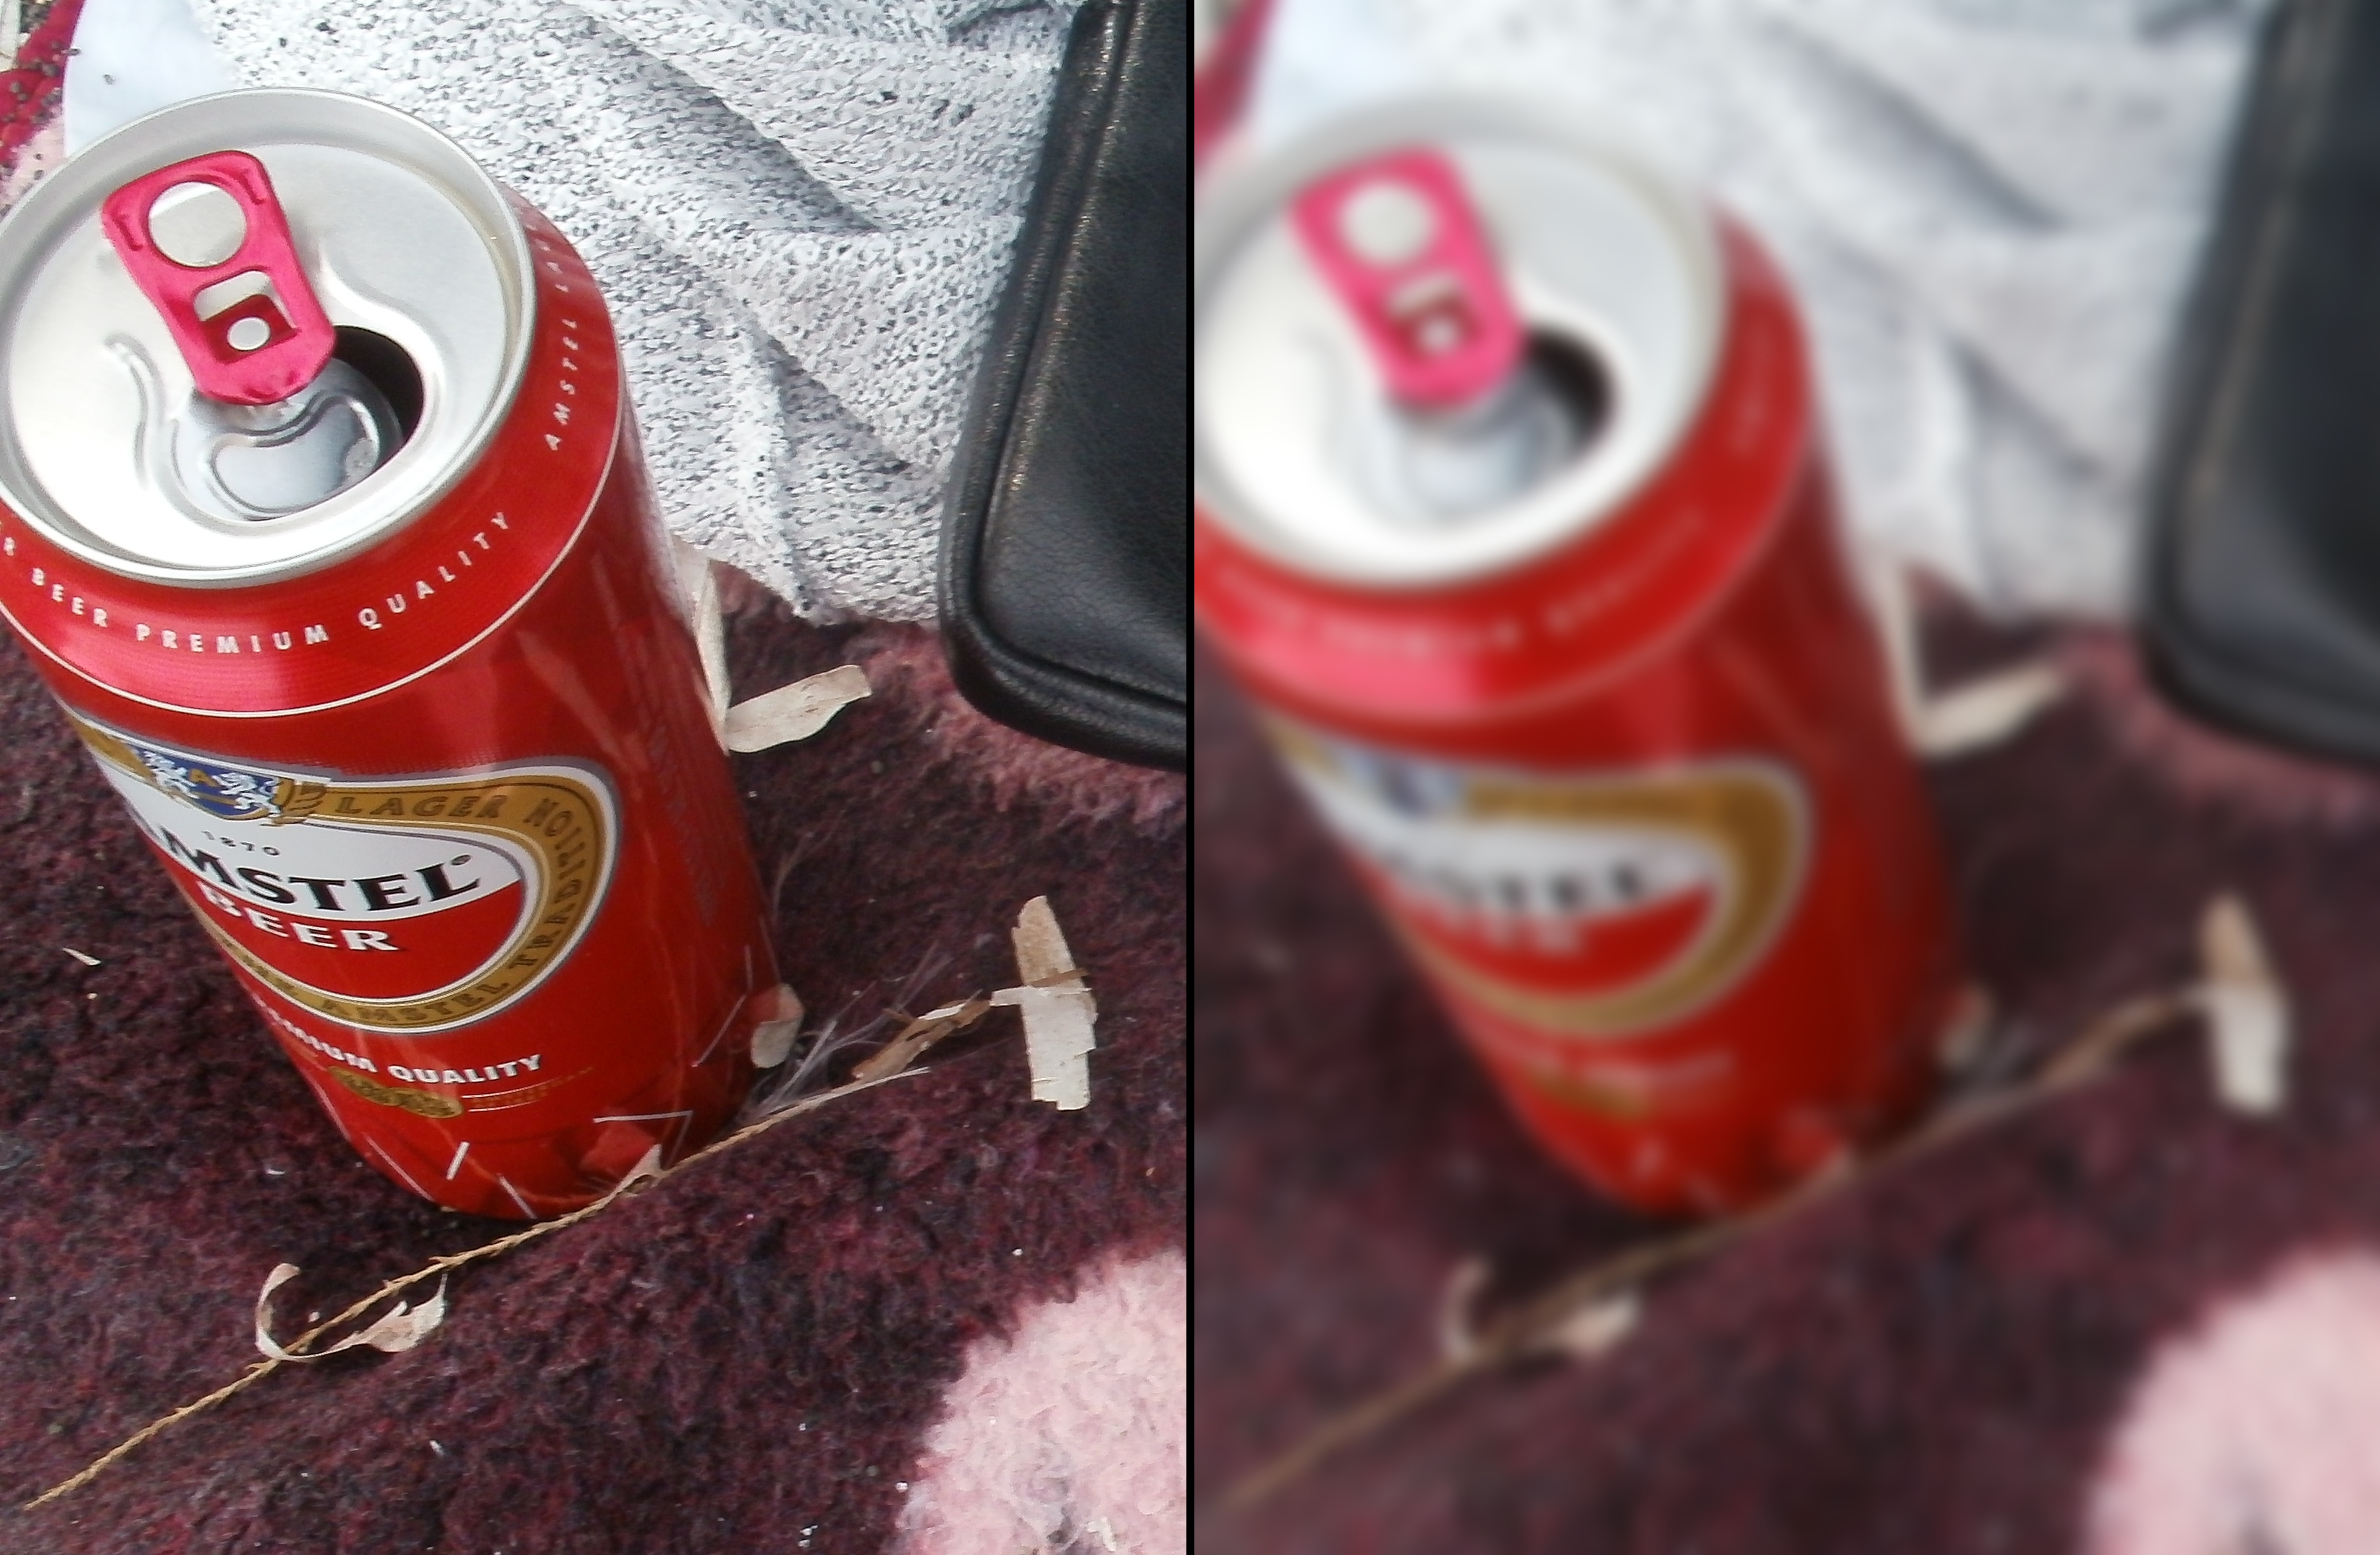
\includegraphics[scale=1.0]{images/GaussianBlurExample.jpg}
\caption{Gaussian Blur example. \\
Source: http://en.wikipedia.org/wiki/File:Halftone,\_Gaussian\_Blur.jpg}
\label{gaussianBlurExample}
\end{center}
\end{figure}

\subsubsection{Bilateral filter}

According to \cite{bilateralFilterWiki}, bilateral filter is a non-linear, edge-preserving and
noise reducing filter for images. The intensity value at each pixel in an image is replaced by a
weighted average of an intensity values from nearby pixels. In contrast to the Gaussian Blur, 
weights are based on the difference of intensity from the center pixel. This algorithm is commonly
used to prepare an input for segmenting algorithms. Algorithm takes three parameters:

\begin{itemize}
  \item \textit{Diameter} of each pixel that is used during filtering. The larger value is set, the
        algorithm is slower and takes into consideration larger pixel surrounding;
  \item \textit{Filter Sigma in a color space}. A larger value of this parameter means, that farther
        colors within the pixel neighborhood will be mixed together. Resulting image will have
        larger areas with semi-equal color;
  \item \textit{Filter Sigma in the coordinate space}. A larger value of the parameter means that
        farther pixels will influence each other as long as their colors are close enough.
\end{itemize}

Example of a bilateral filter usage is presented in a fig.~\ref{bilateralFilterExample}.

\begin{figure}[ht]
\begin{center}
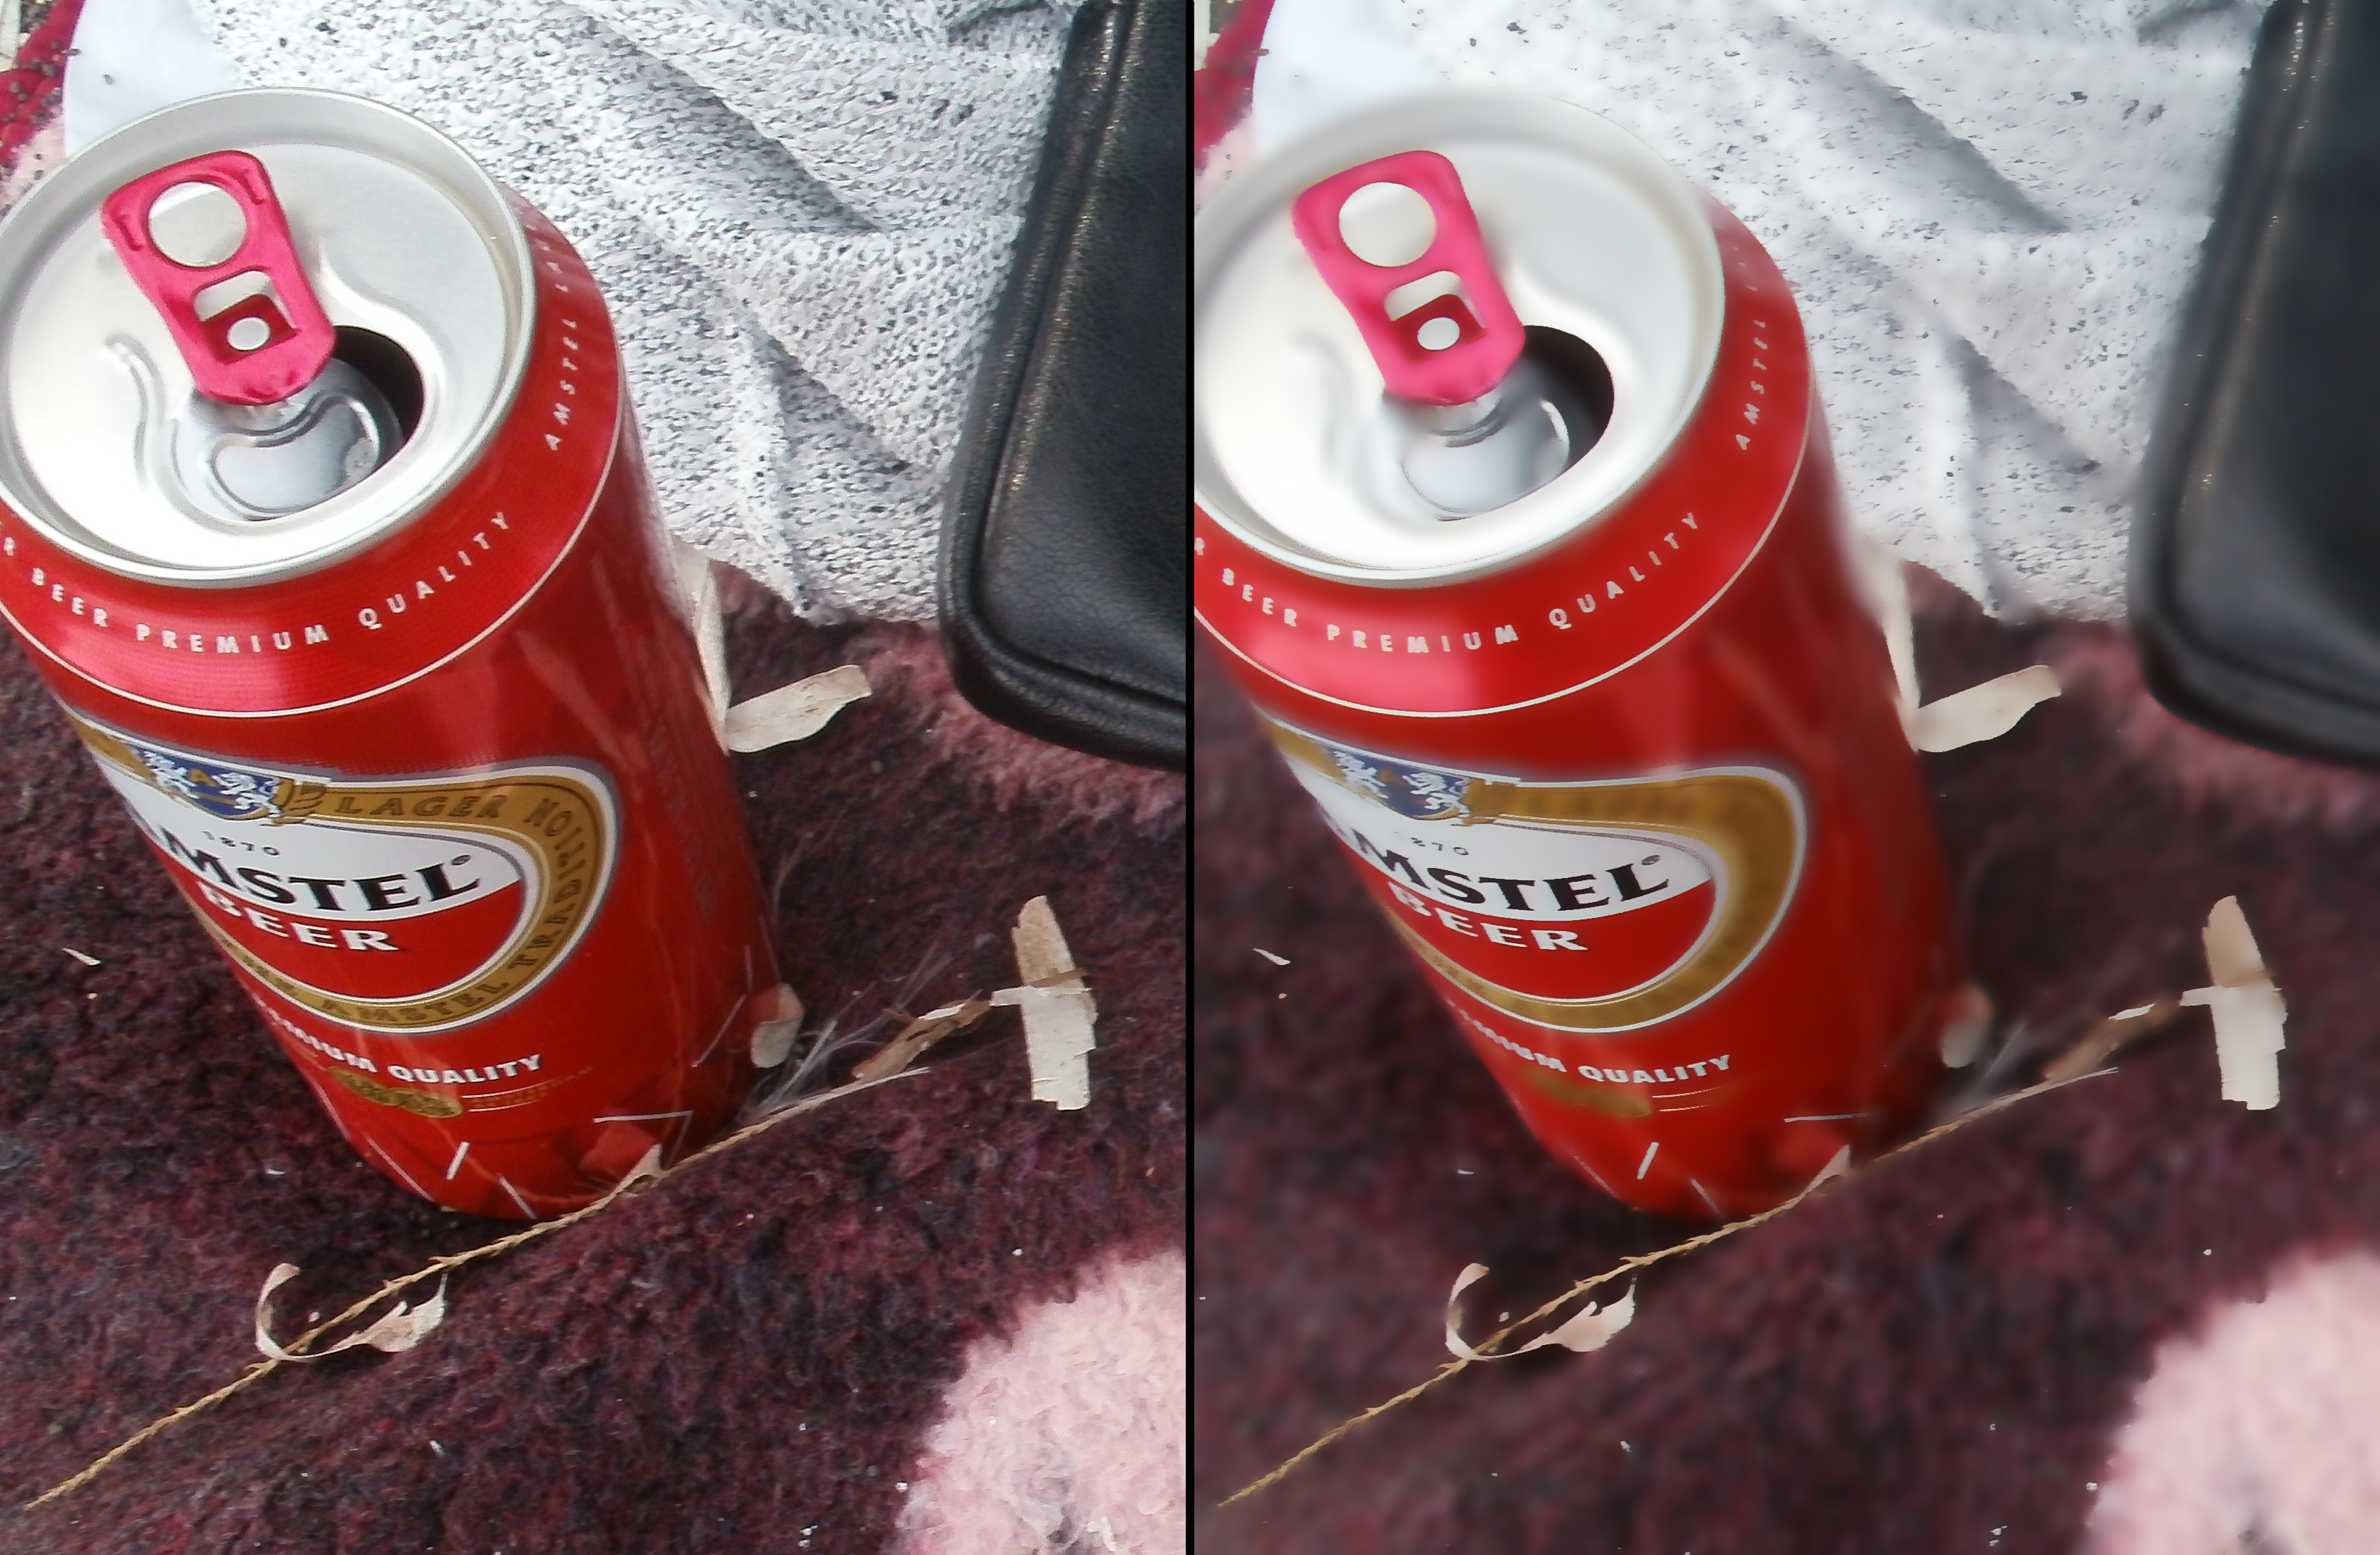
\includegraphics[scale=0.6]{images/BilateralFilterExample.jpg}
\caption{Bilateral Filter example. \\
Source: http://www.planet-source-code.com/Upload\_PSC/ScreenShots/PIC20103161922506817.jpg}
\label{bilateralFilterExample}
\end{center}
\end{figure}

\subsection{Morphological transformations}

Morphological operations are used to remove noise, isolate or joining disparate elements
in an image and find intensity bumps or holes in an image to find image gradients. Basic 
morphological operations are called Dilation and Erosion.

\subsubsection{Dilation}

Dilation is a convolution of an image with a kernel. The kernel can have any shape or size and has
to have defined an anchor point. When kernel is scanned over the image, there is computed maximum
pixel value covered by the kernel. Then, the anchor point value is set to maximum value. Dilation
causes growth of all bright elements in an image. Example of dilation is presented in 
Fig.~\ref{dilationExample}

\begin{figure}[ht]
\begin{center}
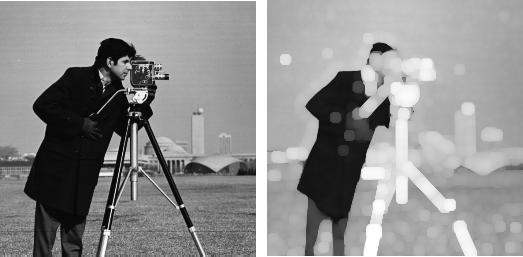
\includegraphics[scale=0.6]{images/dilationExample.jpg}
\caption{Dilation example. \\
Source: http://www.mathworks.com/help/images/ref/referenceipart130.gif}
\label{dilationExample}
\end{center}
\end{figure}

\subsubsection{Erosion}

Erosion is a converse operation to dilation. Main difference is that it computes local minimum over
the area of the kernel. Erosion causes growth of all dark elements in an image. Example of erosion
is presented in Fig.~\ref{erosionExample}

\begin{figure}[ht]
\begin{center}
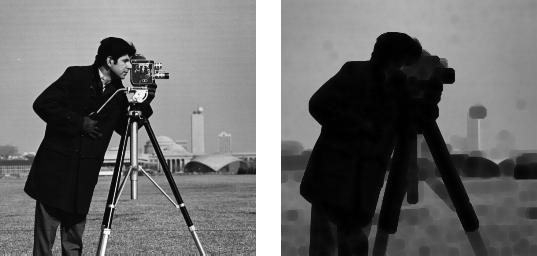
\includegraphics[scale=0.6]{images/erosionExample.jpg}
\caption{Erosion example. \\
Source: http://www.mathworks.com/help/images/ref/referenceipart128.gif}
\label{erosionExample}
\end{center}
\end{figure}

Dilation and erosion take two parameters:

\begin{itemize}
  \item \textit{Size of rectangular structuring element used for erosion/dilation}. If it is set to
        3, the structuring element is a matrix with size 3x3. The bigger value is set, the algorithm
        has stronger impact on the image;
  \item \textit{Number of iterations} of the algorithm.
\end{itemize}

\subsection{Denoising}

Main goal of this type of algorithms is to eliminate noise from the image. In this work algorithm
called Non-local Means Denoising \cite{nonLocalMeansDenoising}. Filter takes one argument. It
regulates the filter strength. Big value of the parameter perfectly removes noise but also removes
image details. Smaller parameter values preserve details but also preserve some noise.
Example of its usage is presented in a Fig.~\ref{denoisingExample}.

\begin{figure}[ht]
\begin{center}
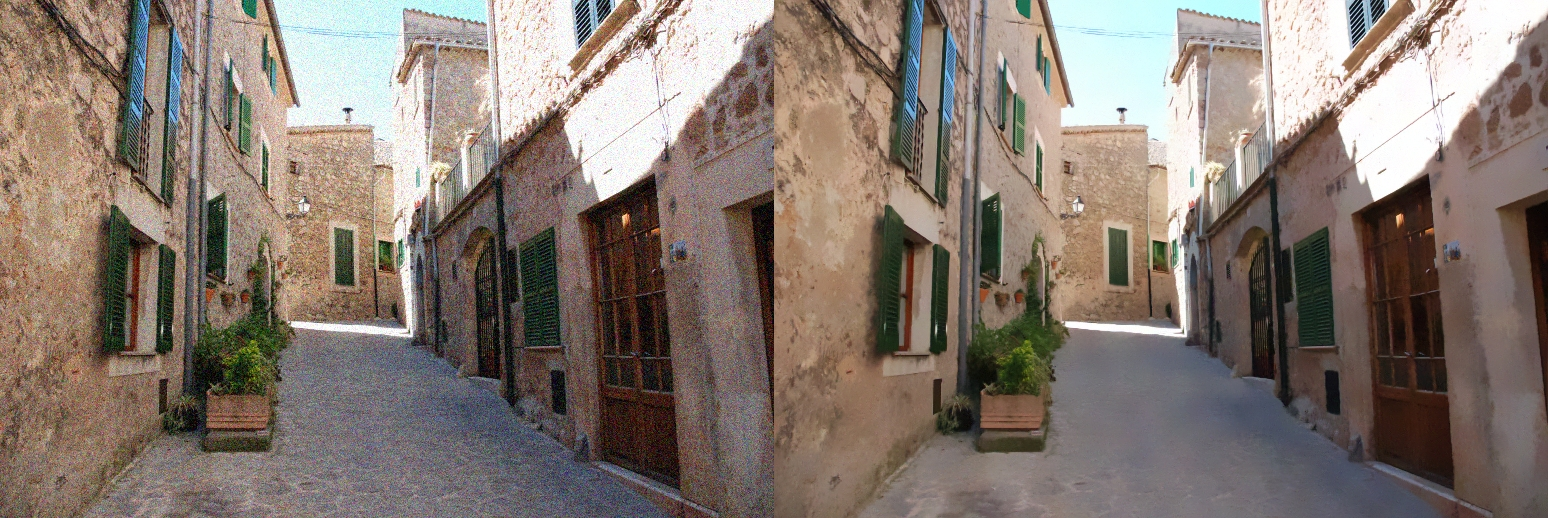
\includegraphics[scale=0.3]{images/denoisingExample.jpg}
\caption{Denoising example. \\
Source: Image generator in \cite{nonLocalMeansDenoising}}
\label{denoisingExample}
\end{center}
\end{figure}

\subsection{Unsharp mask}

Unsharp mask is applied to highlight or enhance some details in an image. According to 
\cite{unsharpMaskWiki}, this technique uses a blured or unsharp image to create mask of the original
image. The unsharped mask is then combined with the negative image. As a result there is an image
less blurry than the original. In algorithm used in this work, Gaussian blur is used and then its
result is compared to the original image. If the difference is greater than specified threshold
value, images are subtracted. Algorithm takes the same arguments, as Gaussian filter. Example of
unsharp mask usage is presented in a Fig.~\ref{unsharpMaskExample}.

\begin{figure}[ht]
\begin{center}
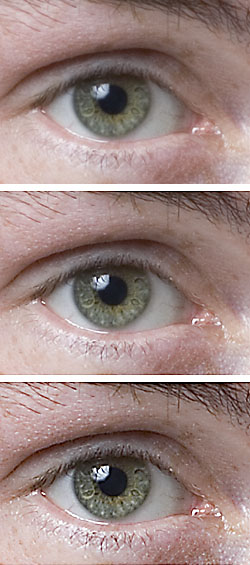
\includegraphics[scale=1.2]{images/unsharpMaskExample.jpg}
\caption{Unsharp mask example. \\
Source: http://upload.wikimedia.org/wikipedia/commons/4/43/Unsharped\_eye.jpg}
\label{unsharpMaskExample}
\end{center}
\end{figure}

\section{Image segmentation}

According to \cite{digitalImageProcessing}, segmentation algorithms partitions images into 
constituent parts or objects. They are generally based on two basic properties of intensity values:
discontinuity and similarity. In first case, the approach is to partition an image based on abrupt
changes in intensity(like for example edges in an image). In second case, the approach is based on
partitioning an image into regions, that are similar(for example they have similar color). There
are many segmentation algorithms available. Solution presented in this work is based on thresholding
approach.

\subsection{Tresholding}

Thresholding, thanks to its properties and simple implementation, is one of the most commonly used
segmentation algorithms. In the most basic form, having gray level of each pixel in an image we can
find a value of threshold, which will separate groups with different gray-level values. Then we 
set appropriate, different color value for pixels, which are above and below threshold value.

Let's assume, that:
\begin{itemize}
  \item T is a threshold value
  \item f(x, y) is a gray-level value in a point x, y
  \item g(x, y) is a thresholded pixel value
\end{itemize}

$$
g(x, y) = \left\{ \begin{array}{ll}
1 & \textrm{if $f(x, y) \geq T$}\\
0 & \textrm{if $f(x, y) < T$}\\
\end{array} \right.
$$

Algorithm takes one parameter - T, which is a thresholding value.

Example image with applied thresholding( with T = 130 ) is presented in a 
Fig.~\ref{thresholdingExample}.

\begin{figure}[ht]
\begin{center}
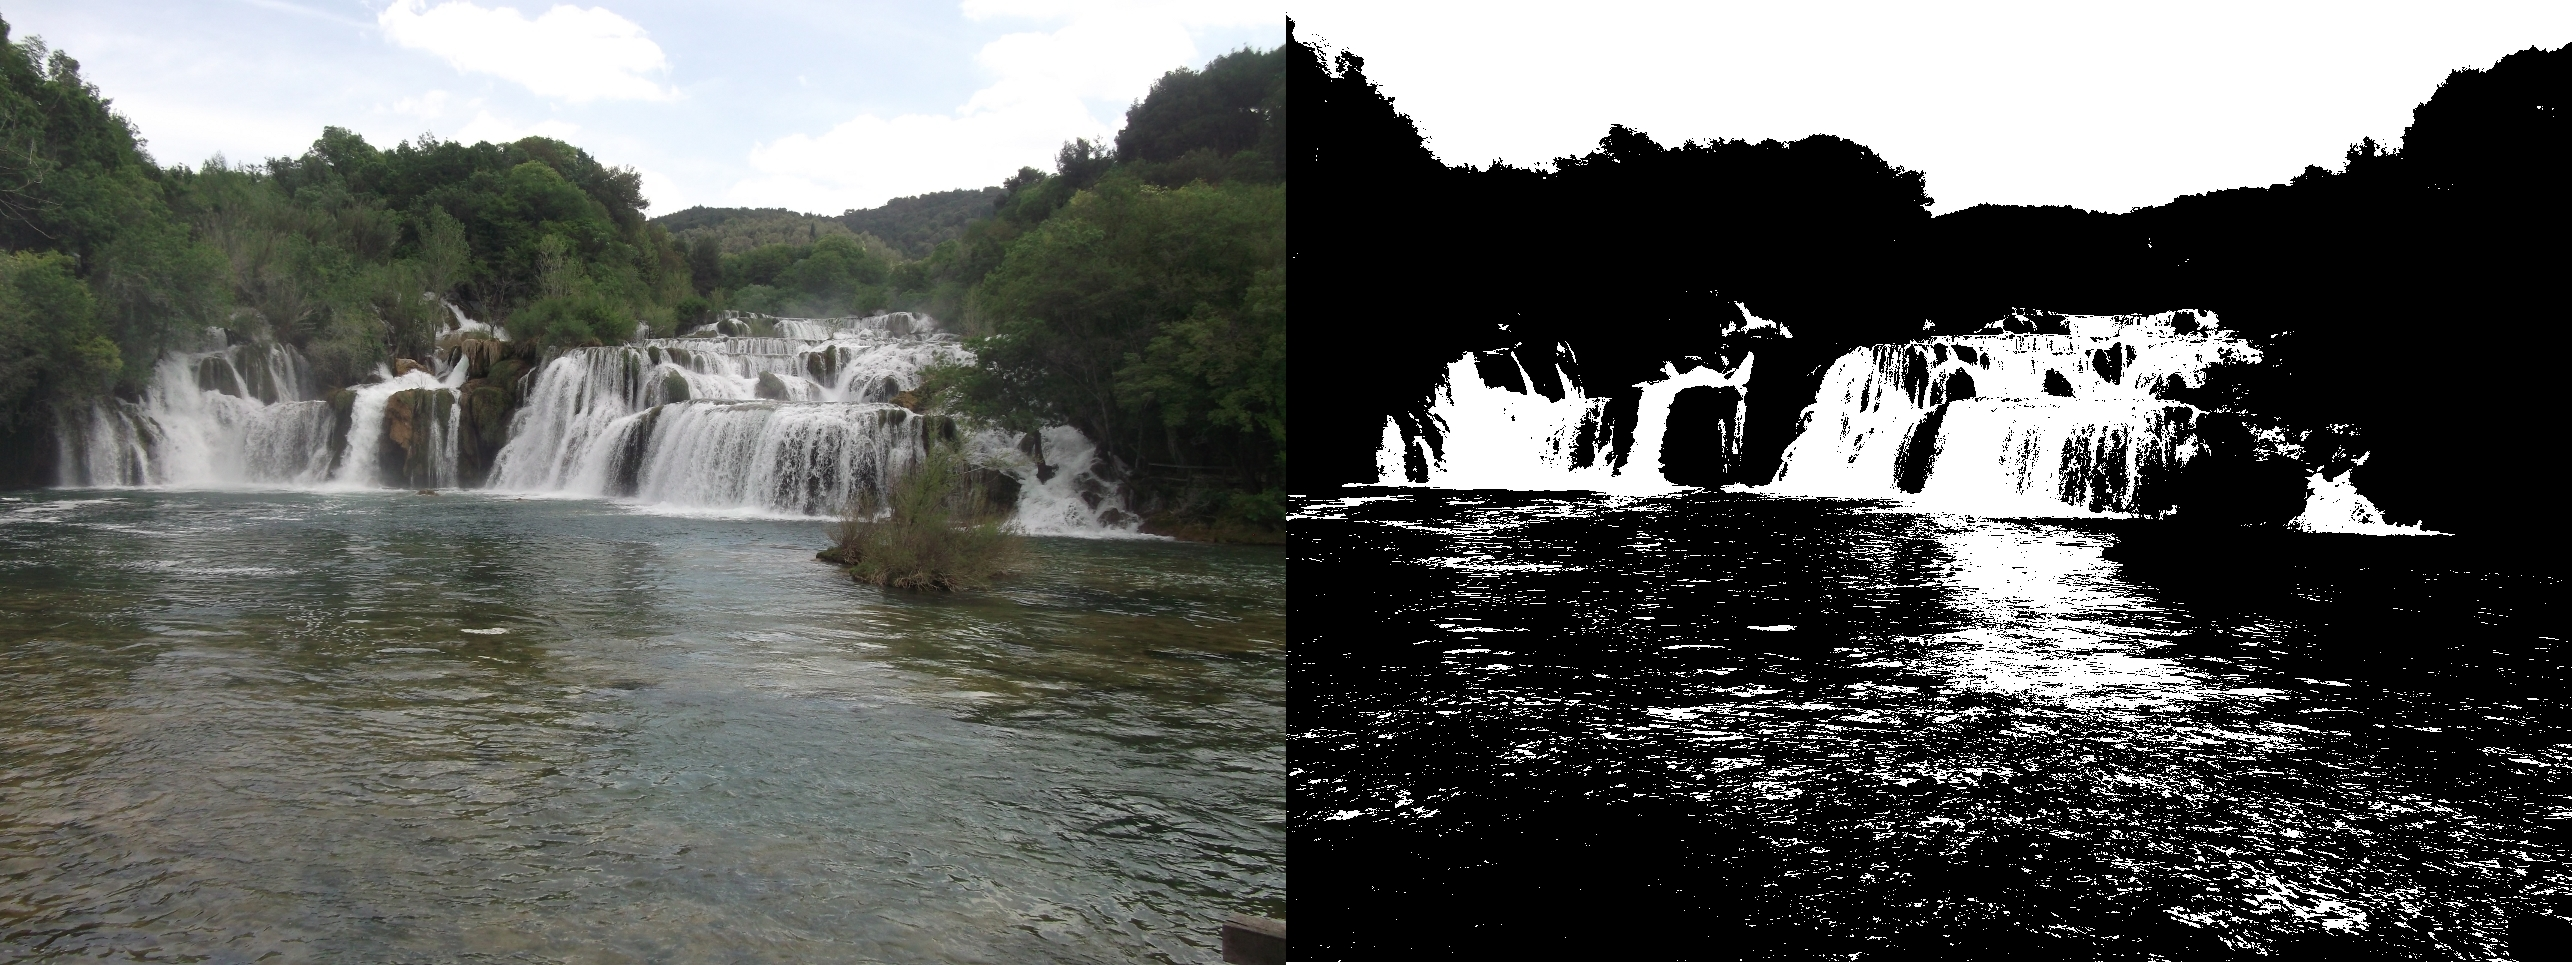
\includegraphics[scale=0.15]{images/thresholdingExample.jpg}
\caption{Thresholding example. \\
Source: own}
\label{thresholdingExample}
\end{center}
\end{figure}

\section{Color scanned maps processing}

Processing of color scanned maps is a very interesting topic. There are some research works focusing
on it. In this section there are short descriptions of found six algorithms, which focus on this
problem.

In \cite{semanticAnalysisAndRecognition}, authors treat alphanumerical signs, letters, points, lines
and areas separately. Image is vectorized and segmented in separate processes. To separate 
alphanumerical characters, there is used a \textit{False Color Technique}. Next, the 
\textit{Composite Image Technique} is used to decompose image and link objects by their associated
names. Finally, set of separate modules grouped as \textit{A2R2V} detect alphanumeric, punctual and
linear characters in the map. In this algorithm there are used such techniques like thresholding,
color segmentation and neural networks.

Another approach is presented in \cite{comparativeAnalysisOfScannedMaps}. This work focused on 
decomposition of scanned topographic maps. Algorithm finds different areas(like lakes, rivers,
contours, text, grid and other) using map analysis and thresholding in a black and white mode.
Next, there are used filtering algorithms to remove elements smaller than expected and noise.
Then map texture is analysed. This step is helpful in detection of areas like for example lakes.
Algorithm uses thresholding, median filter and many color segmentation techniques.

Next method is shown in \cite{colorsOfThePast}. Authors of this research worked with maps from 
19th century. The algorithm is divided into four stages. First, the clustering algorithm allows 
automatic determination of the pixels, which represent color layer prototypes uin three domains:
local image domain, histogram analysis and color space. In second phase, pixels are defined as
layer specific seeds based on distances in color space to the color points of the computed layer 
prototypes and local homogenity. Third phase takes the result of previous part and it identifies 
connected regions of pixels belonging to one of the color layers. Finally, unallocated pixels are
joined to proper groups.

Another solution is presented in \cite{automaticVectorization}. This work is focused on segmentation
of contour maps. There are used \textit{Deformable Model Tracking} and \textit{Adaptive Flow 
Orientation}. It uses a seed segment searching and variable force control. Contour lines are 
detected automatically. This method is good at detection of crossed, broken and touching lines.

Next algorithm can be found in \cite{topographicMapsAutomaticVectorization}. In this work image is
segmented with a "Peeling Onion Strategy". Layers are recognized separately. Each recognized layer
is subtracted of the map to facilitate the interpreation of remaining, more complex ones. Sequence
of processes is as follows:

\begin{itemize}
  \item Recognition of objects for which there is external data available;
  \item Recognition and vectorization of textured areas;
  \item Recognition of strings and symbols;
  \item Recognition of objects with variable shape;
  \item Recognition of networks.
\end{itemize}

In these processes there are used pattern matching, contour following, polygonal approximation and
skeletonization algorithms, 

Last presented approach is shown in \cite{colorMapSegmentation}. There is presented a segmentation
method dedicated for United States Geological Survey(U.S.G.S.) topographic maps. Algorithm first 
segments out white background. Next, image is segmented using Eigenvector line fitting technique.
Algorithm knows typical values of colors used in U.S.G.S. In the final part of the algorithm, proper
color value is set for every pixel(it is based on distance of pixel Eigenvector and Eigenvalue and
a known value of known U.S.G.S. colors). Summarizing, the segmentation algorithm uses knowledge
about colors used in maps from U.S.G.S.

\chapter{Research design}

In this chapter there is a full description of an algorithm processing scanned maps. Additionaly,
there is a description of an input data and found problems related to it.

\section{Input data description}

Algorithm has two inputs. One is a file containing an image with a map. Second input is a
configuration file, which contains parameters of an algorithm.

\subsection{Map image file}

Input of the algorithm is an digital image, stored in a disk in one of many available formats, like
png, tif, jpg or bmp. Image should be a color-scanned map at any resolution. Example image is 
presented in a Fig.~\ref{inputExample}. It is a scanned color map of a Polish city - Brzeg.

\begin{figure}[!ht]
\begin{center}
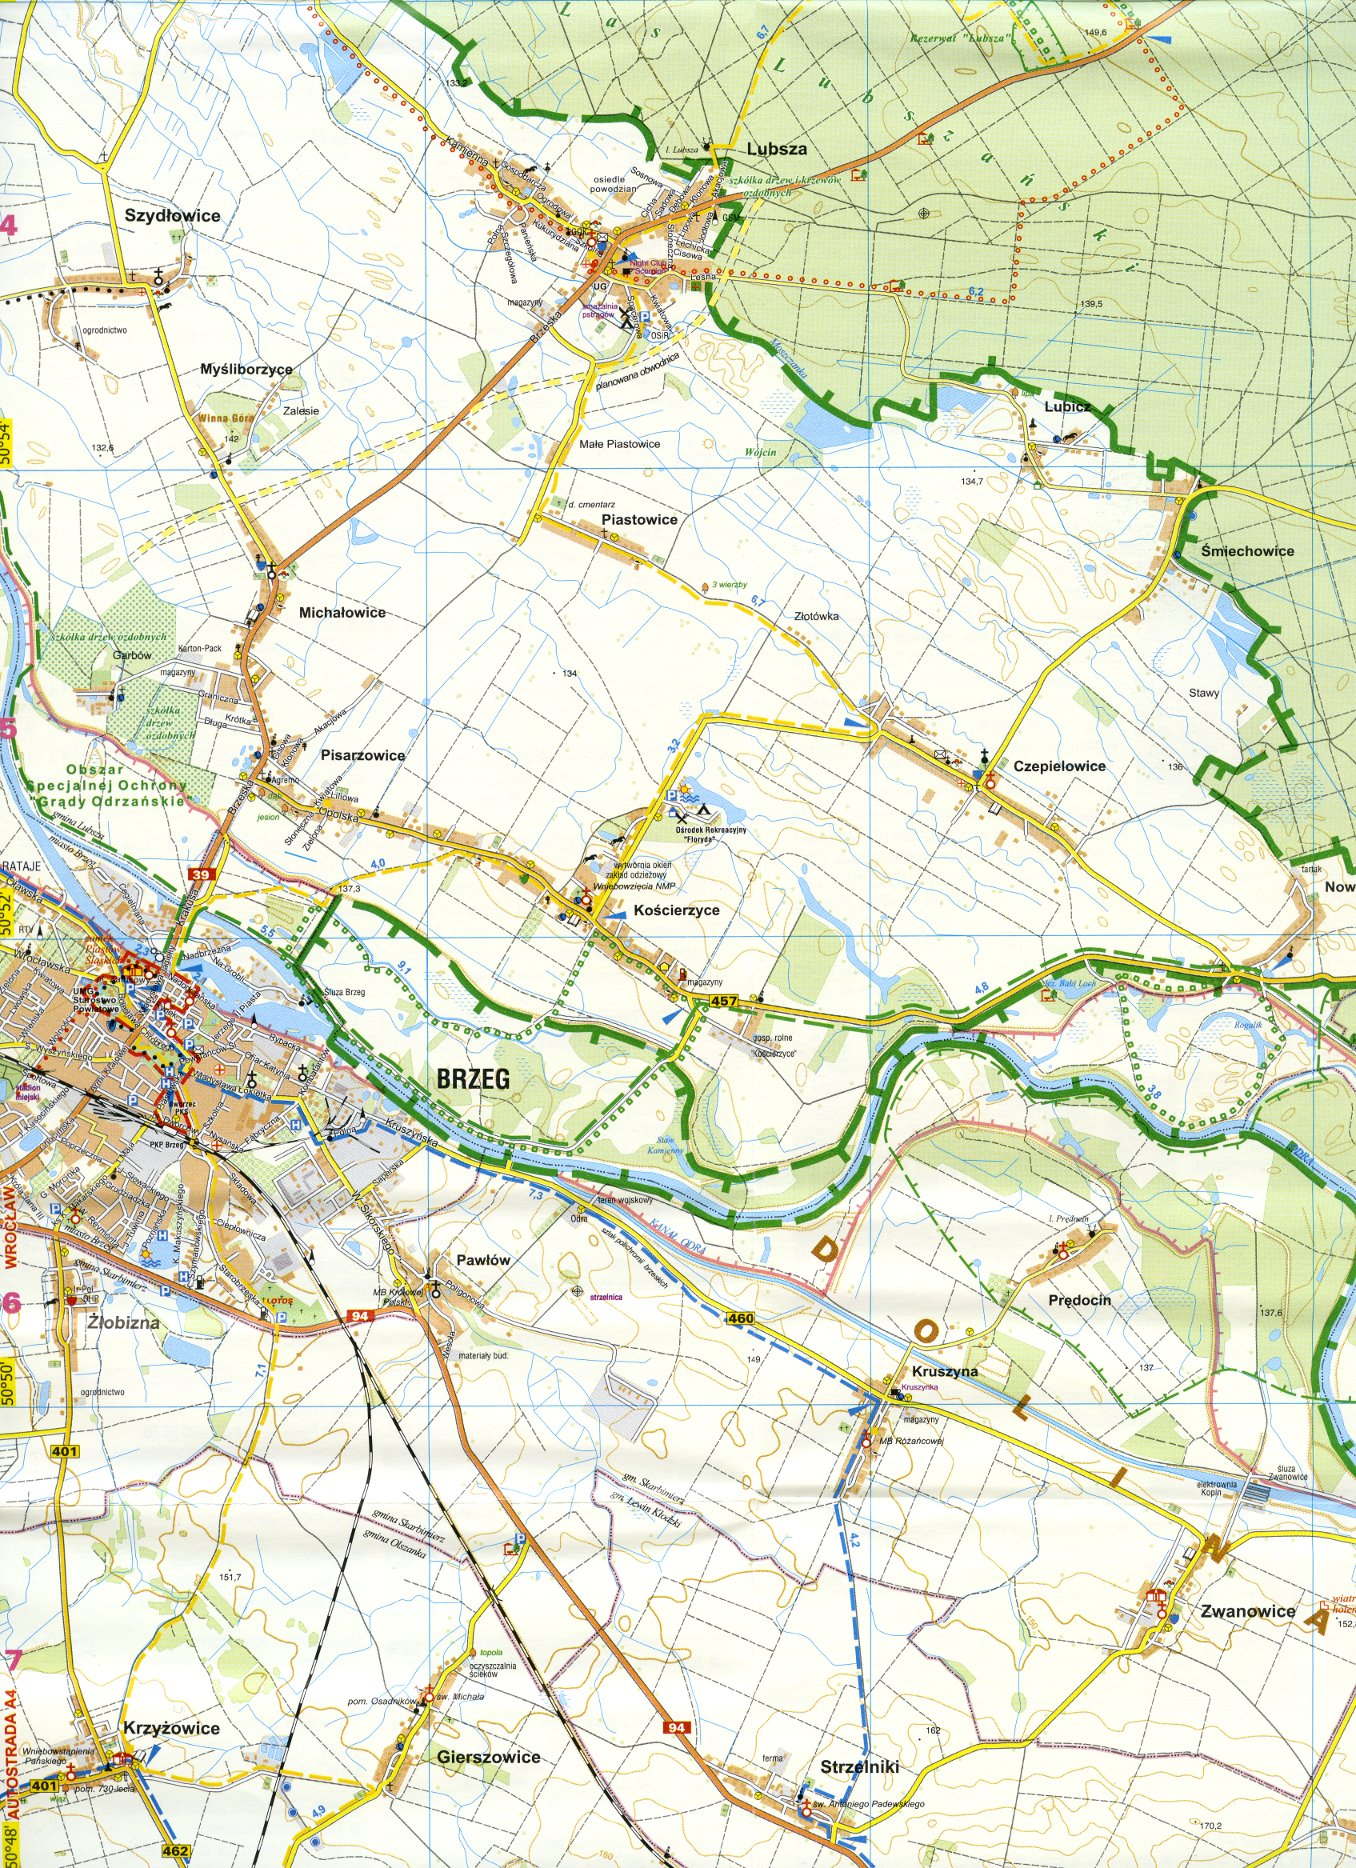
\includegraphics[scale=0.78]{images/brzeg.jpg}
\caption{Example input.}
\label{inputExample}
\end{center}
\end{figure}

To confirm proper working of the algorithm, there were nine maps prepared. All input map files
with its description are listed in a table~\ref{tableInputFiles}. 

\begin{table}[!ht]
\begin{center}
\caption{Input files.}
\label{tableInputFiles}
\begin{tabular}{|c|c|c|c|}
  \hline
  Filename & Format & Resolution & Description \\
  \hline
  brzeg & tif & 3391x4671 & Map of Brzeg. It has text and multiple areas like \\
        &     &           & forests, lakes, roads and cities \\
  \hline
  bydgoszcz & bmp & 1747x1272 & Map of Bydgoszcz. Small number of areas, \\
            &     &           & high density of roads and small details \\
  \hline
  dolny\_slask & png & 5936x8669 & Old map of a Lower Silesia. No backround. \\
              &     &           & Many thin lines and rivers. \\
  \hline
  lubsza & tif & 3391x4671 & Map of surroundings of Lubsza. It has many areas \\
         &     &           & like forests and lakes. Image has a big damage. \\
         &     &           & Map was bent during scanning process. \\
  \hline
  masyw\_slezy & tif & 3883x4606 & Topographic map of Ślęża Mountain. It contains \\
              &     &           & many areas in different colors, roads, text and \\
              &     &           & topographic lines. \\
  \hline
  namyslow & jpg & 4814x5628 & Topographic map of Namysłów. It contains many \\
           &     &           & small details, topographic lines, small text  \\
           &     &           & and bright background of areas\\
  \hline
  pokoj & tif & 2921x2989 & Map of Pokój. It has text, multiple areas \\
        &     &           & (forests, lakes) and roads. \\
  \hline
  sleza & jpg & 1812x2756 & Map of Ślęża. It contains areas like forests, \\
        &     &           & lakes and roads. \\
  \hline
  sobotka & png & 2798x1824 & Map of Sobótka. It has many different areas, like \\
          &     &           & small details, text and roads. \\
  \hline
\end{tabular}
\end{center}
\end{table}

\subsection{Configuration file}

Created algorithm has number of parameters, which have to be determined. Application loads them
using special XML file. Parameters in a configuration file are divided to two layers. Meaning
and usage of each parameter is explained in next sections. Example XML configuration file is
listed in~\ref{listingConfig}

\begin{lstlisting}[caption=Example configuration XML file,label=listingConfig,language=xml]
<?xml version="1.0" encoding="UTF-8"?>
<configuration>
    <background_detection>
        <enabled>true</enabled>
        <gaussian_blur_radius>9</gaussian_blur_radius>
        <gaussian_blur_standard_deviation>0</gaussian_blur_standard_deviation>
        <diameter>20</diameter>
        <sigma_color>150</sigma_color>
        <sigma_space>150</sigma_space>
        <dilation_and_erosion_size>2</dilation_and_erosion_size>
        <dilation_and_erosion_counter>4</dilation_and_erosion_counter>
        <window_width>15</window_width>
        <max_number_of_colors>30</max_number_of_colors>
    </background_detection>
    <line_detection>
        <enabled>true</enabled>
        <threshold_value>100</threshold_value>
        <unsharp_mask_standard_deviation>5</unsharp_mask_standard_deviation>
        <denoising_factor>35</denoising_factor>
        <bilateral_filter_counter>5</bilateral_filter_counter>
        <gaussian_blur_radius>5</gaussian_blur_radius>
        <gaussian_blur_standard_deviation>0</gaussian_blur_standard_deviation>
        <gaussian_blur_counter>2</gaussian_blur_counter>
        <initial_threshold>10</initial_threshold>
        <mimimal_color_area>500</mimimal_color_area>
        <max_number_of_colors>15</max_number_of_colors>
        <diameter>20</diameter>
        <sigma_color>75</sigma_color>
        <sigma_space>50</sigma_space>
    </line_detection>
</configuration>
\end{lstlisting}

\section{Problems and restrictions}

There are a lot of problems associated with segmentation of scanned maps. Due to imperfection of
a scanning process, resulting color scanned digital images have many distortions.
There are also problems connected with input image(it can be damaged before scanning).
Moreover, raster derived from printed document should be removed.
Additionaly maps have many small elements and text. These details, as well as shape of background
areas (like for example lakes and forests) should be kept in resulting image.
All found problems are described more precisely in next sections.

\subsection{Input image and scanning process quality}

Scanned digital images have many distortions. They are related with damage of an input image, like
places, where maps are creased(example in Fig.~\ref{creaseExample}) or dirty(shown in a 
Fig.~\ref{dirtyExample}). It results in the existence of darker elements in the output image.

\begin{figure}[!ht]
\begin{center}
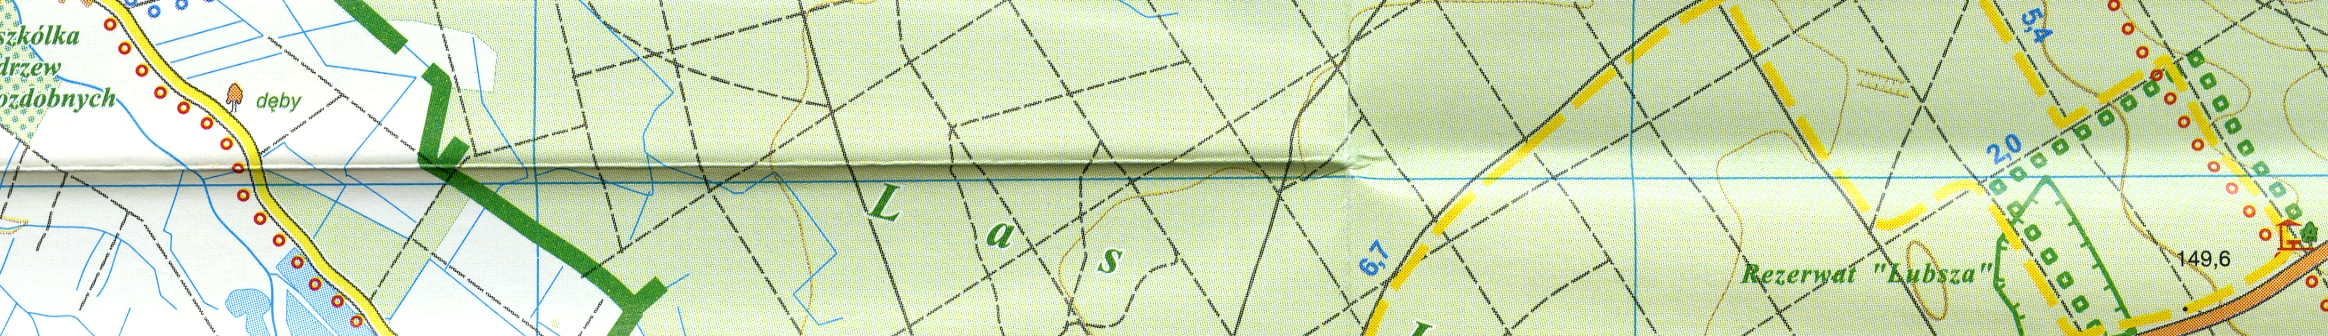
\includegraphics[scale=1.1]{images/creaseExample.jpg}
\caption{Example of distortion caused by creased maps.}
\label{creaseExample}
\end{center}
\end{figure}

\newpage

\begin{figure}[!ht]
\begin{center}
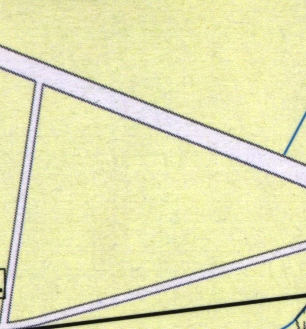
\includegraphics[scale=3.0]{images/dirtyExample.jpg}
\caption{Example of distortion caused by dirty map.}
\label{dirtyExample}
\end{center}
\end{figure}

Another problems are related to scanning process. Resulting images are noisy. Additionaly a
scanning device or scanned map can be dusty. These problems results in small distortions, which
should not be placed in an output image. Example of this situation is presented in a 
Fig.~\ref{dustExample}. It is marked in red rectangle.

\begin{figure}[!ht]
\begin{center}
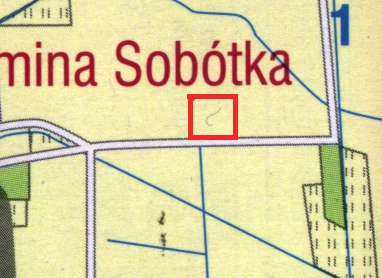
\includegraphics[scale=3.0]{images/dustExample.jpg}
\caption{Example of distortion caused by dust.}
\label{dustExample}
\end{center}
\end{figure}

Finally, resulting image can have undesirable areas with wrong(usually darker) color. Their
existence is caused by mistakes made during scanning process, for example when image is not properly
put in a scanner surface. This situation is visualized in a Fig.~\ref{badScanExample}.

\begin{figure}[!ht]
\begin{center}
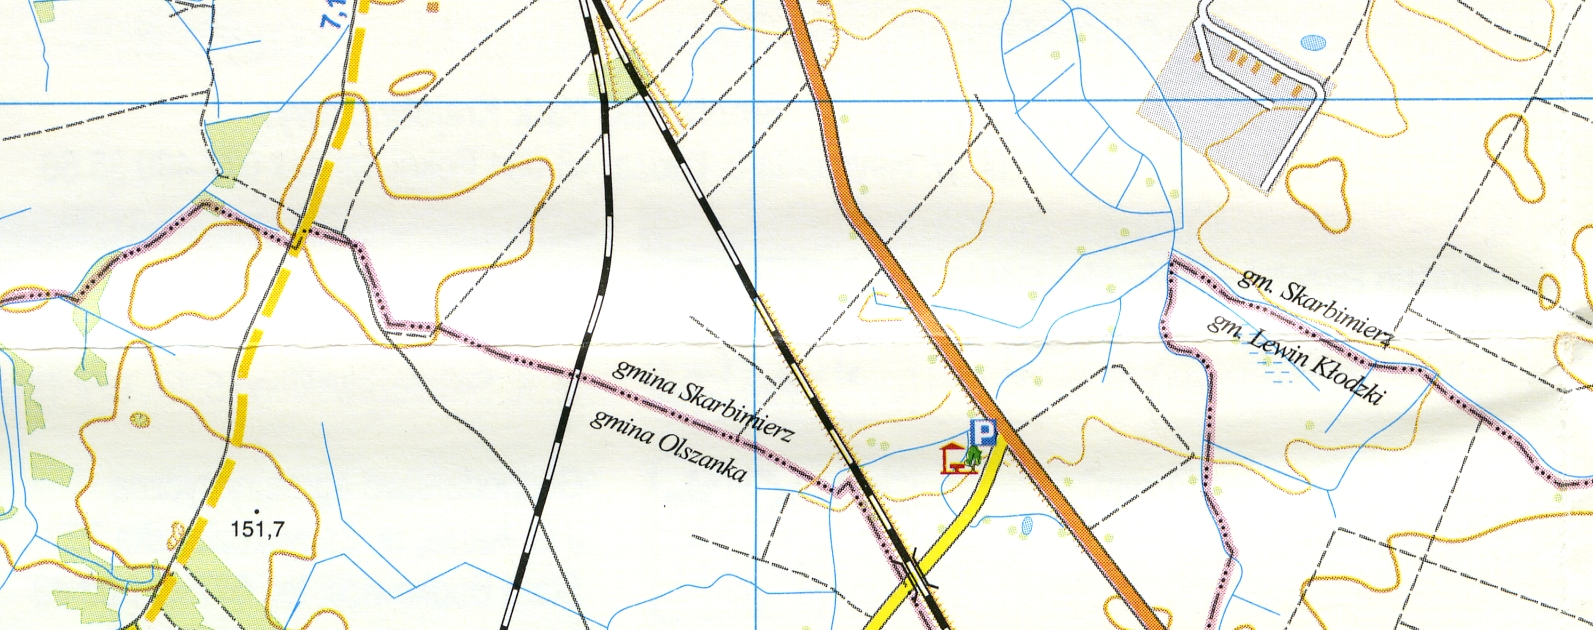
\includegraphics[scale=1.3]{images/badScanExample.jpg}
\caption{Example of distortion caused by improper scanning.}
\label{badScanExample}
\end{center}
\end{figure}

\subsection{Small details}

Input image contains many small details. They exist especially in city and topographic maps.
City maps contain a lot of small elements, like churches, parking places or gas stations.
Additionaly, in cities there are many roads and areas, which are marked in different colors. 
Furthermore they contain many small letters, which, for example, indicate names of streets, parks
or major buildings and places. Finally, in the city map, lines, roads and test are 
often crossing each other. Example fragment of a city map fragment is shown in a 
Fig.~\ref{cityExample}.

\begin{figure}[!ht]
\begin{center}
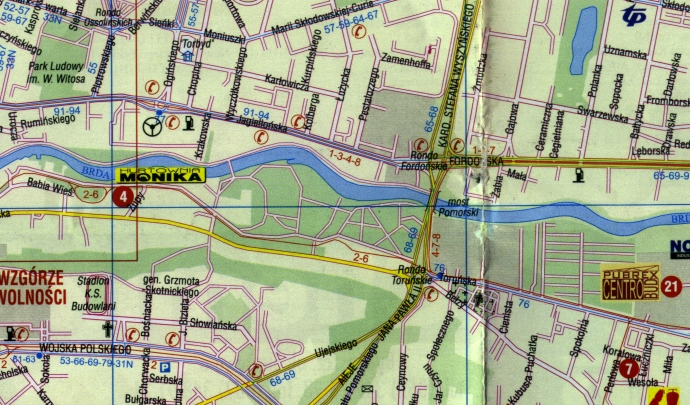
\includegraphics[scale=0.65]{images/cityExample.jpg}
\caption{Fragment of a map with a city.}
\label{cityExample}
\end{center}
\end{figure}

Another problems are in topographic maps. They have small letters and elements in different
colors. Additionaly they contain very thin topographic maps. Many of them are not continuous
(some lines are even marked as dots in the same color). These problems are shown in a fragment of a
topographic map in a Fig.~\ref{topographicMapExample}.

\begin{figure}[!ht]
\begin{center}
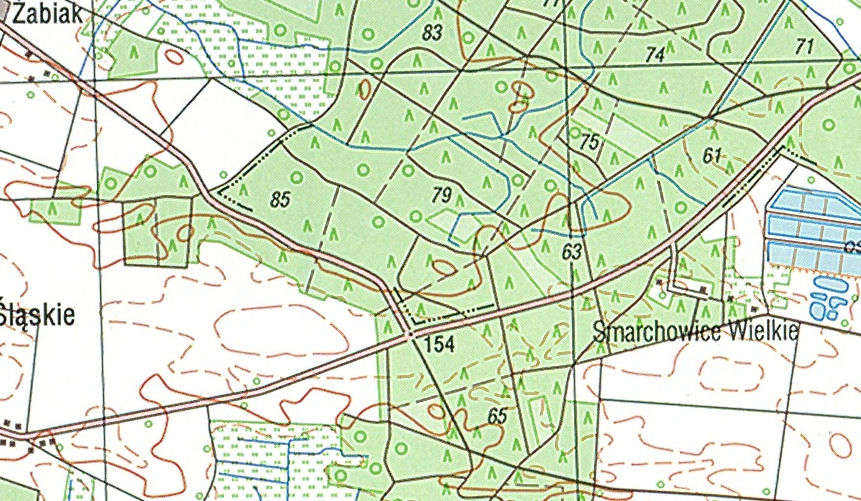
\includegraphics[scale=2.0]{images/topographicMapExample.jpg}
\caption{Fragment of a topographic map.}
\label{topographicMapExample}
\end{center}
\end{figure}

\subsection{Raster elimination}

Digital image coming from a scanner is a raster image. Every pixel is defined itself. This
representation has some disadvantages. One of them is called moro effect. It interferes with
segmentation algorithm. Example of a moro effect is shown in a Fig.~\ref{moroEffectExample}

\begin{figure}[!ht]
\begin{center}
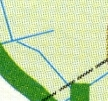
\includegraphics[scale=11.0]{images/moroEffectExample.jpg}
\caption{Example of a moro effect.}
\label{moroEffectExample}
\end{center}
\end{figure}

\section{Main parts of the algorithm}

Map segmentation is a complicated process. In the one hand, all background with as small number of
mistakes as possible should be segmented. To reduce scanning errors and unifize background, many 
smoothing algorithms can be applied, like for example Gaussian Filter. On the other hand there are a
lot of details, lines and text like for example streets, toponyms, symbols and topographic lines.
In this case using smoothing algorithms with bigger parameters is not a good idea - these algorithms
cause, that for example text is deformed and not as sharp as in the input image. To solve these
problems, algorithm has been divided into two parts. First one is responsible for detection of all
details(roads, text, lines, rivers). Second one detects background of the map. Both algorithms work
independently and take as an input the same, input image. They can work simultaneously. Results of
segmentation of both layers are merged to one output image. Flow of the algorithm is presented on a
statechart in a Fig.~\ref{algorithmParts}.

\begin{figure}[!ht]
\begin{center}
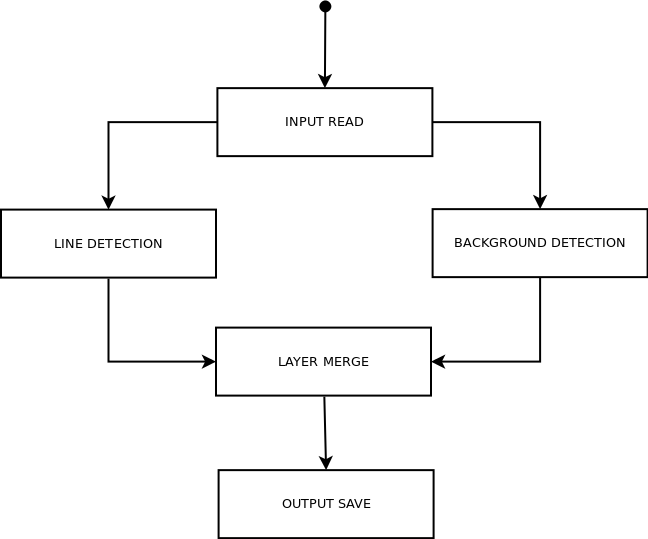
\includegraphics[scale=0.5]{images/allAlgorithmParts.png}
\caption{Parts of the algorithm.}
\label{algorithmParts}
\end{center}
\end{figure}

\section{Detection of areas}

The main aim of this part is to detect all background elements, like for example lakes, forests and
thicker lines(rivers, main roads). The algorithm focuses on elimination of all distortions and
on detection and unification of color of areas. This method should remove all thiner lines and small
details from an image. In an output image there should appear background elements. Every separate
area should have a different color. Main distortions should be eliminated.

\subsection{Algorithm parts}

The algorithm firstly applies a group of algorithms to remove some distortions and prepare image for
a final segmentation. In this case there are used some smoothing algorithms, like Gaussian Filter
and Bilateral Filter. Then, smaller details are eliminated. To do that, there are used Dilation and
Erosion algorithms. In the next step image is segmented. Main aim of this part is to unify color for
each area. Finally, areas with too small area are eliminated from an output image. They are
substituted with colors of areas, which are around them. Flow of the background detection algorithm
is presented in a Fig.~\ref{backgroundDetectionImage}

\begin{figure}[!ht]
\begin{center}
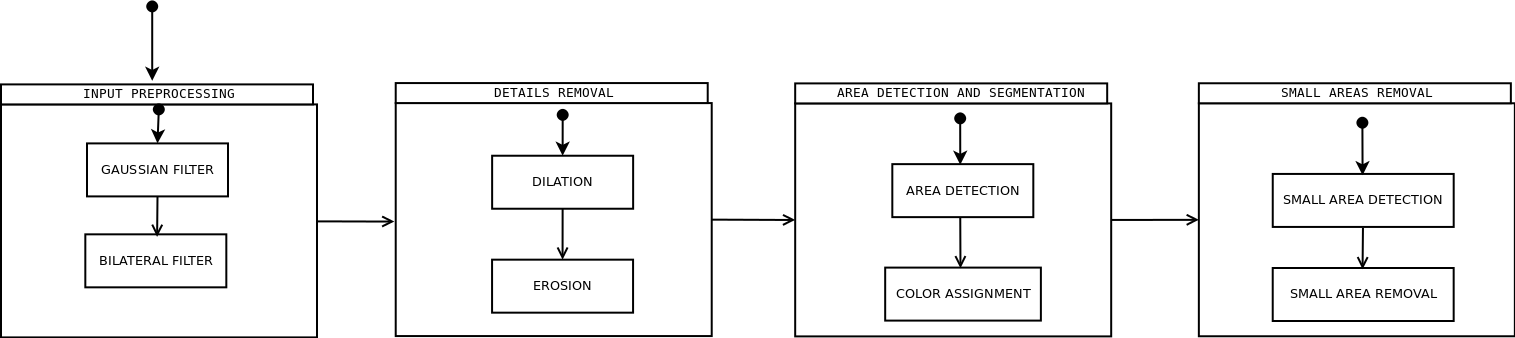
\includegraphics[scale=0.3]{images/backgroundDetection.png}
\caption{Background detection process.}
\label{backgroundDetectionImage}
\end{center}
\end{figure}

\subsubsection{Input preprocessing}

In an input preprocessing part there were used two algorithms: \textit{Gaussian Filter} and \textit{
Bilateral Filter}. Usage of first one is a very good method in elimination of raster and small
distortions(like for example dust). The algorithm is called with a big value of \textit{Radius}
parameter - it helps to remove more distortions, loss of image sharpness is irrelevant in this
case. In a Fig.~\ref{gaussianBlurResult} there is an example usage of a Gaussian Filter with 
\textit{Radius} = 5. All major distortions and moro effect do not exist in a resulting image.
Sharpness of the text(in this case name of the river) is lost.

\begin{figure}[!ht]
\begin{center}
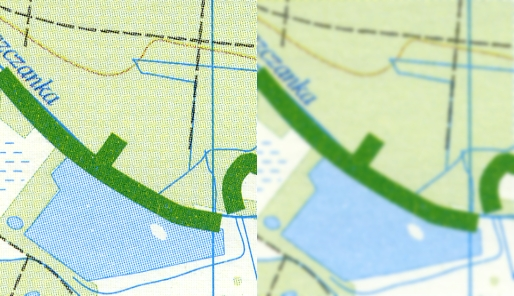
\includegraphics[scale=3.0]{images/GaussianBlurResult.jpg}
\caption{Fragment of a map of Brzeg with Gaussian Blur with Radius = 5 applied. \\ 
Original image is on the left. On the right side there is a resulting image.}
\label{gaussianBlurResult}
\end{center}
\end{figure}

Second algorithm - bilateral filter reduces noise, which was visible in an input map. It has also
another advantage - all edges are kept. In case of a background detection, similarly to Gaussian
Filter, large values of parameters are used. It causes, that a bilateral filter has a big influence
on resulting image. Colors of all areas are aligned. In a Fig.~\ref{bilateralFilterResult}, there is
an example result of applying bilateral filter. Colors of green area, border line, roads and a town
are aligned. Some small details dissapeared.

\begin{figure}[!ht]
\begin{center}
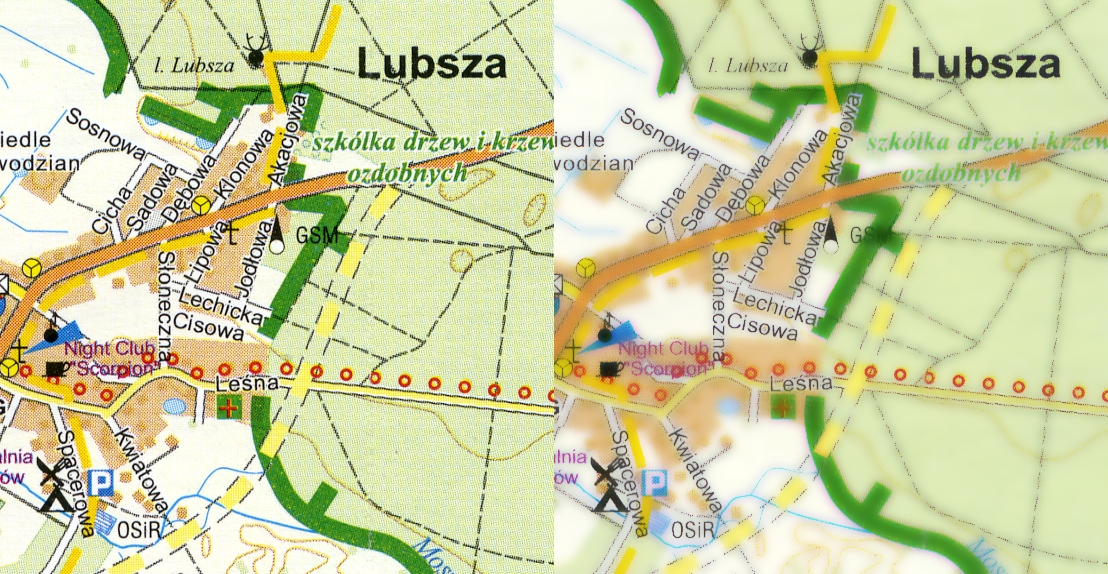
\includegraphics[scale=1.5]{images/BilateralFilterResult.jpg}
\caption{Fragment of a map of Brzeg with Bilateral Filter with Diameter = 30 and Delta values = 150
applied. Original image is on the left. On the right side there is a resulting image.}
\label{bilateralFilterResult}
\end{center}
\end{figure}

\subsubsection{Removal of details}

Erosion and Dilation algorithms are useful in removing noise, joining or isolation of individual
elements and finding intensity holes or bumps in an image. Thanks to these properties, it is easy
to eliminate unwanted, small elements from an image, like roads, rivers, small details(in cities) or
topographic lines. These algorithms are helpful in removal of some distortions of a map, like for
example darker areas caused by unproper scanning process or map creases - image after applying these
algorithms have these unwanted areas eliminated. Usage of dilation cause, that all thin areas
dissapear. Furthermore, distance of every separate element grows.

\begin{figure}[!ht]
\begin{center}
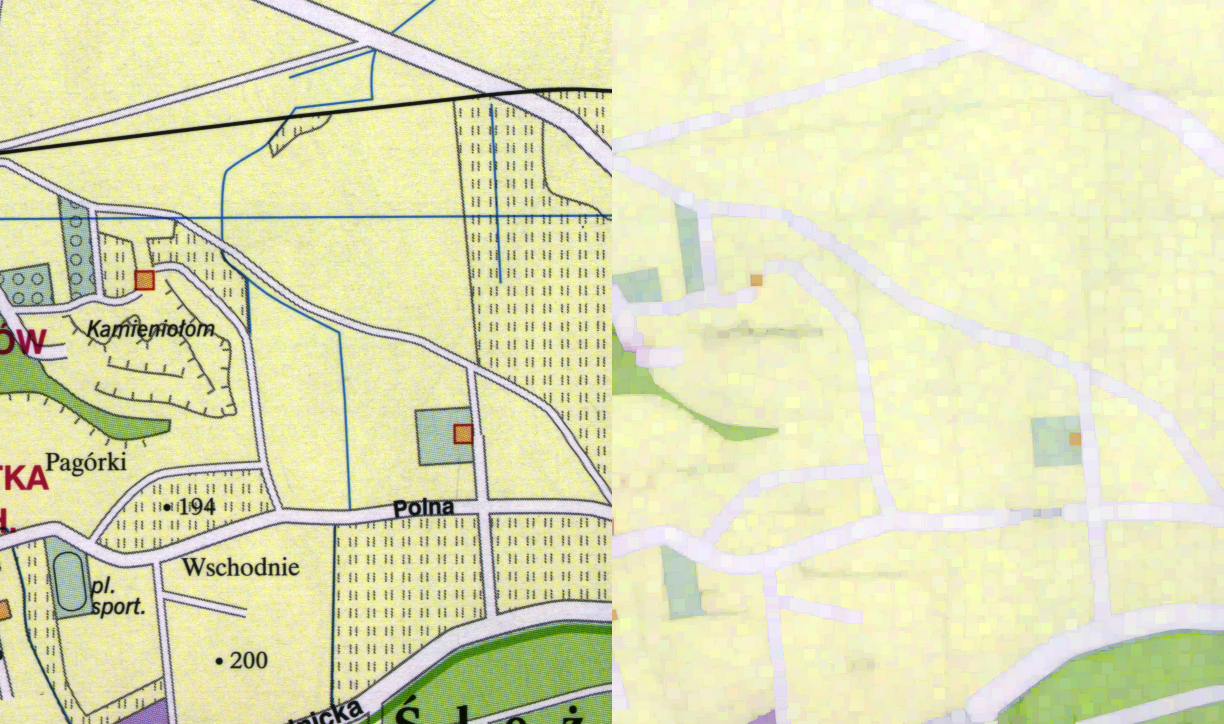
\includegraphics[scale=1.0]{images/dilationResult.png}
\caption{Fragment of a map of Sobótka with dilation applied(5 times). \\
Original image is on the left. On the right side there is a resulting image.}
\label{dilationResult}
\end{center}
\end{figure}

Example of dilation usage is in a Fig.~\ref{dilationResult}. All thin lines are eliminated from the
resulting image. In the output there are visible only yellow and green backgrounds(with some
distortions eliminated). Moreover there is a background of roads and areas of three smaller
elements.

Erosion does the opposite - it causes, that all lines become thicker. It also merges broken
elements. Example of its use is in a Fig.~\ref{erosionResult}. Every line is thicker than in the
original. Borders of every area is easy to determine. Colors of areas are darker and unified.

\begin{figure}[!ht]
\begin{center}
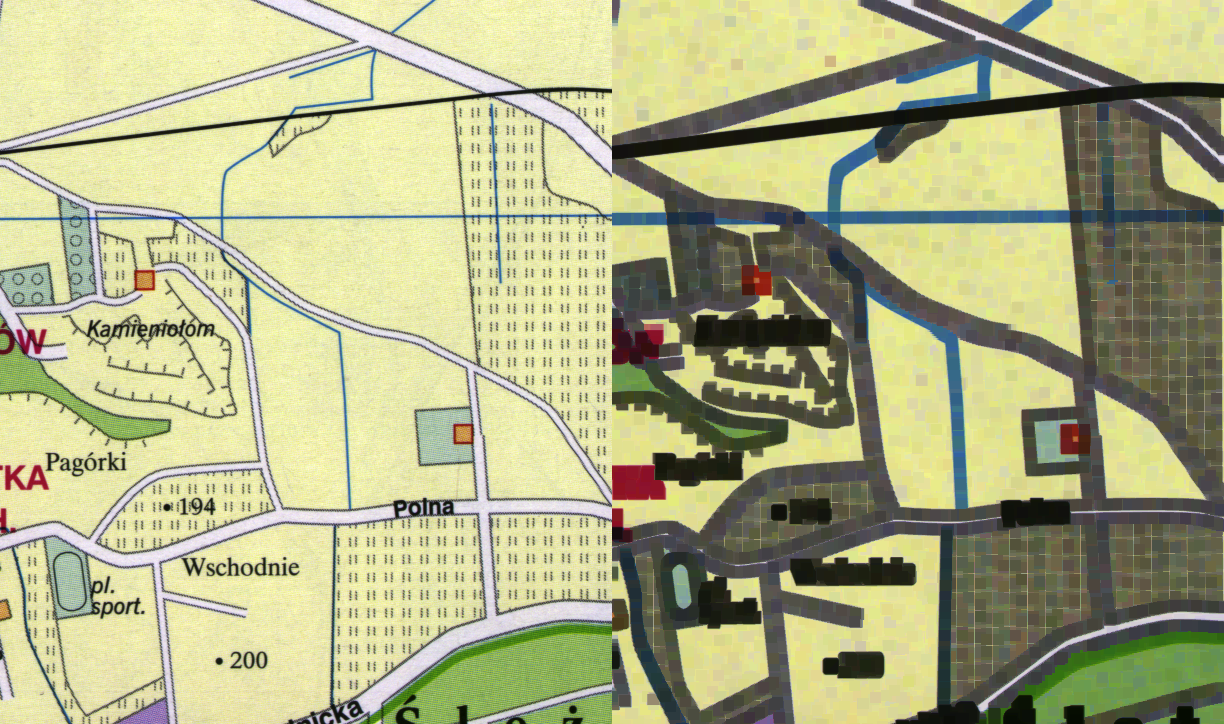
\includegraphics[scale=1.0]{images/erosionResult.png}
\caption{Fragment of a map of Sobótka with erosion applied(5 times). Original image is on the left.
On the right side there is a resulting image.}
\label{erosionResult}
\end{center}
\end{figure}

In case of background detection in scanned color maps, these algorithms give the best results when
they are combined together. After applying these operations, noise and all smaller elements(listed
above) are removed. Major distortions are also eliminated. Moreover colors of every area is almost
the same. As a result, these algorithms are an excellent base for segmentation methods. Example
usage of combined dilation and erosion is presented in a Fig.~\ref{dilationErosionResult}. Every
area has different color and output image have unnecessary details eliminated.

\begin{figure}[!ht]
\begin{center}
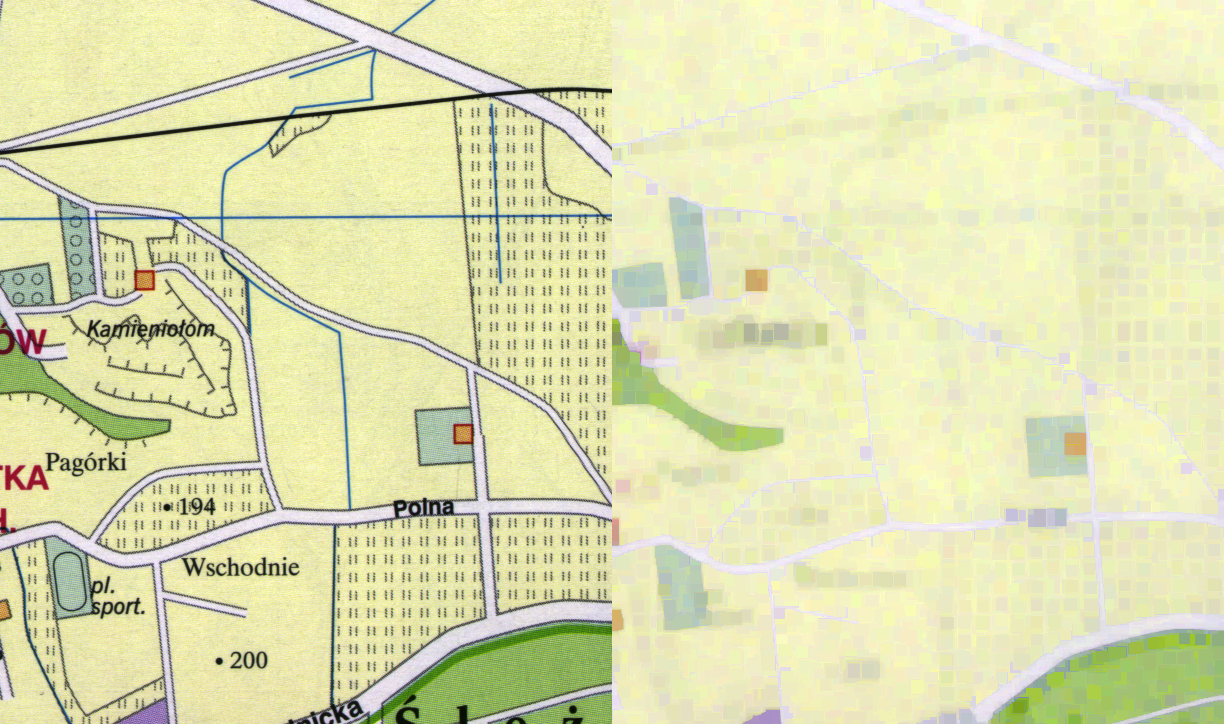
\includegraphics[scale=1.0]{images/dilationErosionResult.png}
\caption{Fragment of a map of Sobótka with dilation(5 times) and then erosion(also 5 times) applied.
Original image is on the left. On the right side there is a resulting image.}
\label{dilationErosionResult}
\end{center}
\end{figure}

\subsubsection{Areas detection and segmentation}

Detection of all map areas is based on two properties. First one is color of every group represented
by their pixels. Second one is a desired number of areas, which should be detected(this number is
easy to determine in case of digital maps). The algorithm at the beggining analyses each pixel of an
image and groups them. As a result there are groups of pixels with similar color. In the next step,
all groups, which represent similar values are merged until the desired number of colors is reached.
In the last part, each pixel of an image is assigned to best-fitting group. The whole process with
its parameters is described in Algorithms~\ref{colorGroupingAlgorithm},~\ref{groupsMergingAlgorithm}
~and~\ref{colorAssignmentAlgorithm}. \\

Parameters of the algorithm:
\begin{itemize}
  \item \textit{Threshold} - The maximum distance between the currently checked color and a group,
          determining if the color should be assigned into group
  \item \textit{Maximum Number of Colors}, which determines, how much groups should exist in an
          output map(the actual number of background colors in a map)
\end{itemize}

\begin{algorithm}[!ht]
  \KwData{Threshold}
  \KwIn{Image}
  \KwOut{Colors grouped by color similarity}

  GroupContainer gc\;
  \ForEach{Pixel in Image}
  {
    pixelAddedToGroup := false\;
    \ForEach{Group in gc}
    {
      \If{distance(Pixel.color, Group.averageColor) < Threshold}
      {
        Group.add(Pixel)\;
        pixelAddedToGroup := true;
      }
    }

    \If{pixelAddedToGroup = false}
    {
      gc.createNewGroup(Pixel)\;
    }
  }

  \Return{gc}

  \caption{Color grouping}
  \label{colorGroupingAlgorithm}
\end{algorithm}

\begin{algorithm}[!ht]
  \KwData{Threshold}
  \KwData{MaximumNumberOfColors}
  \KwIn{GroupContainer gc}
  \KwOut{SegmentedImage}

  \Repeat{gc.numberOfGroups > MaximumNumberOfColors}
  {
    \ForEach{Group in gc}
    {
      \ForEach{AnotherGroup in gc}
      {
        \If{distance(Group.averageColor, AnotherGroup.averageColor) < Threshold)}
        {
          mergeGroups\;
        }
      }
    }
    Threshold := Threshold + 1\;
  }

  \Return{gc}

  \caption{Groups merging}
  \label{groupsMergingAlgorithm}
\end{algorithm}

\begin{algorithm}[!ht]
  \KwIn{GroupContainer gc}
  \KwIn{Image}
  \KwOut{SegmentedImage}

  \ForEach{Pixel in Image}
  {
    group := gc.getBestFittingGroup{Pixel}\;
    Pixel.color := group.averageColor\;
  }

  \Return{Image}

  \caption{Color assignment}
  \label{colorAssignmentAlgorithm}
\end{algorithm}

The distance between colors is Euclidean:~
$$
distance(c1, c2) = \sqrt{(c1.red - c2.red)^2 + (c1.green - c2.green)^2 + (c1.blue - c2.blue)^2}
$$

The color of entire group is counted as average value of red, green and blue of every pixel
belonging to this group. The best fitting group for a pixel is that one, which distance to the pixel
is the smallest.

\begin{figure}[!ht]
\begin{center}
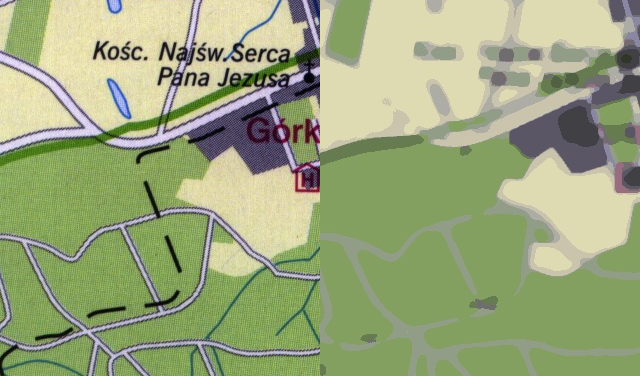
\includegraphics[scale=2.5]{images/segmentationResult.png}
\caption{Fragment of a map of Ślęża with segmentation algorithm applied.
Original image is on the left. On the right side there is a resulting image.}
\label{segmentationResult}
\end{center}
\end{figure}

In a Fig.~\ref{segmentationResult}, there is an example result of applying the segmentation
algorithm. There was used preprocessed(with filtration, dilation and erosion) map of Ślęża. Initial
threshold was set to 30, maximum number of colors was set to 20. Each area has its unified color.
Shape of every area is fairly kept. There are some small areas, which have assigned wrong color.
They exist mainly in places, where there was text in the input image.

\subsubsection{Removal of small areas}

After segmentation of areas in the map, there are often some pixels, which were interpreted as a
wrong area. It is easy to detect this situation, because wrongly assigned pixels are in most of
cases surrounded by properly evaluated elements. To remove such misinterpreted pixels, the Holes
Removal algorithm has been designed. This method investigates surrounding of each pixel in an image.
New color of the pixel is set to the value, which is the most frequent in the surrounding area.
Algorithm has one parameter - it is a size of the matrix, which surrounds the pixel. This matrix is
used for the analysis of color of area, which is around processed pixel. The bigger value is set,
the bigger area is taken into consideration. For example, for parameter value = 7, the surrounding
area is a matrix with a size 7x7. Pseudocode of the algorithm is presented in
\ref{holesRemovalAlgorithm}.

\begin{algorithm}[!ht]
  \KwIn{WindowWidth}
  \KwIn{Image}
  \KwOut{SegmentedImage}

  \ForEach{Pixel in Image}
  {
    window := getWindow(windowWidth)\;
    newColor := window.getMostFrequentColor\;
    pixel.color := newColor\;
  }

  \Return{Image}

  \caption{Holes removal}
  \label{holesRemovalAlgorithm}
\end{algorithm}

In a Fig.~\ref{holeRemovalResult}, there is presetend example usage of Holes Removal algorithm. It
was applied to previously segmented map of Ślęża. Solution has been applied with a Window Width
parameter set to a very big value - 50. The resulting image has all distortions eliminated.
Unfortunately proper edges and sizes of areas have been lost. It follows, that used window width
parameter value was too big. The bigger value of Window Width argument is used, the more details
are eliminated and also there is bigger risk to loose backround borders.

\begin{figure}[!ht]
\begin{center}
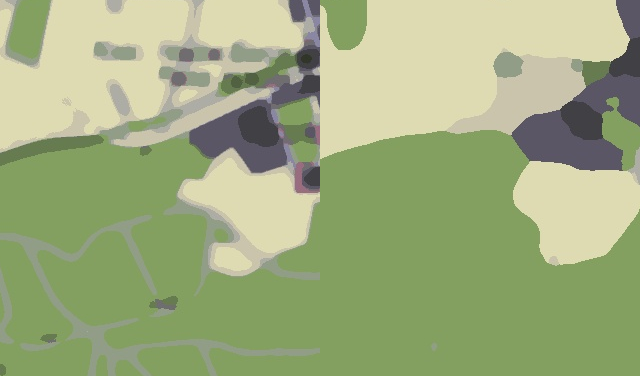
\includegraphics[scale=0.5]{images/holeRemovalResult.png}
\caption{Fragment of a map of Ślęża with Holes Removal algorithm applied.
On the left, there is an image after segmentation. On the right side there is an image with removed
holes.}
\label{holeRemovalResult}
\end{center}
\end{figure}

\subsection{Algorithm parameters}

There are some arguments, which have to be set before application of the algorithm. Their values
depend on the map, to which algorithm is applied. To achieve the best results, every map should have
individually set of parameter values.

\begin{description}
  \item[enabled] \hfill \\
    Determines, if Background Detection algorithm is enabled. \\
    Possible~values:~\{\textit{true},~\textit{false}\};
  \item[gaussian\_blur\_radius] \hfill \\
    Radius of a Gaussian Blur. \\
    Possible~values:~integer number. Proposed~values:~[5~-~15];
  \item[gaussian\_blur\_standard\_deviation] \hfill \\
    Standard deviation of a Gaussian Blur. \\
    Possible~values:~integer number. Proposed~values:~[0~-~5];
  \item[diameter] \hfill \\
    Diameter used by Bilateral Filter. \\
    Possible~values:~integer number. Proposed~values:~[10~-~30];
  \item[sigma\_color] \hfill \\
    Sigma Color used by Bilateral Filter. \\
    Possible~values:~integer number. Proposed~values:~[50~-~150];
  \item[sigma\_space] \hfill \\
    Sigma Space used by Bilateral Filter. \\
    Possible~values:~integer number. Proposed~values:~[50~-~150];
  \item[dilation\_and\_erosion\_size] \hfill \\
    Size of rectangular structuring element used in erosion in dilation algorithms. \\
    Possible~values:~integer number. Proposed~values:~[1-10];
  \item[dilation\_and\_erosion\_counter] \hfill \\
    Number of erosion and dilation applications. \\
    Possible~values:~integer number. Proposed~values:~[2~-~10];
  \item[window\_width] \hfill \\
    Width of a window used by Holes Removal algorithm. \\
    Possible~values:~integer number. Proposed~values:~[5~-~15];
  \item[max\_number\_of\_colors] \hfill \\
    Maximal number of colors, which should be visible in resulting map. \\
    Possible~values:~integer number. Proposed~values:~[10~-~50].
\end{description}

\section{Detection of details}

The main aim of this part of the algorithm is to detect and unify smaller elements, which exist in
the map. These are for example:
\begin{itemize}
  \item thin lines like for example streets, roads, rivers, topographic lines, etc.;
  \item Strings: toponyms and other text, names of the streets;
  \item Small elements from the legend, like for example churches, parking places.
\end{itemize}

The algorithm focuses mainly on filtering out the background, detecting all types of elements and
finally, classification of every detected element or line to one of previously discovered groups.
The result of this part should be an image with isolated and properly classified all map details.

\subsection{Algorithm parts}

In the first part, the algorithm tries to remove all background from the map and keep only wanted
details. In this case there is thresholding algorithm used. Next, there is applied algorithm, which
removes all distortions resulting from thresholding algorithm. This part there is called a 
procedure, which finds and removes all single occuring(lonely) pixels. In the next part, there is
applied an unsharp mask to improve image quality. Finally, all elements are recognized and 
classified to appropriate group. Flow of the entire algorithm is presented in a 
Fig.~\ref{detailDetectionFlow}.

\begin{figure}[!ht]
\begin{center}
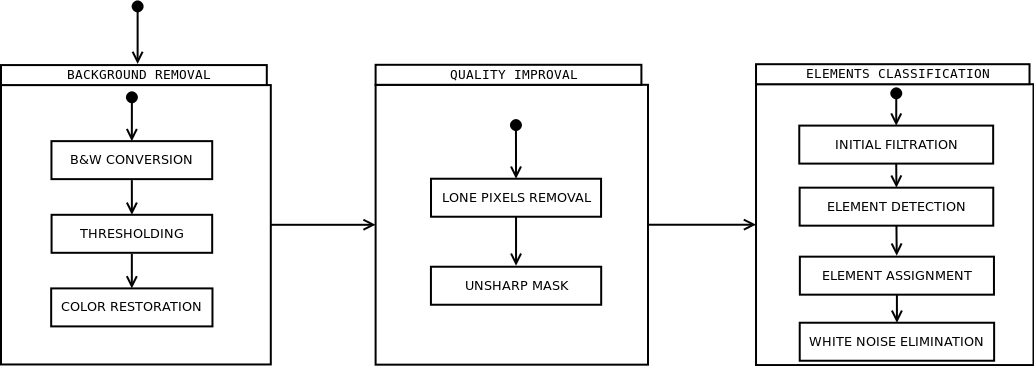
\includegraphics[scale=0.4]{images/detailDetectionFlow.png}
\caption{Flow of the Detail Detection algorithm}
\label{detailDetectionFlow}
\end{center}
\end{figure}

\subsubsection{Background removal}



\subsubsection{Quality improval}

\subsubsection{Elements classification}

\subsection{Algorithm parameters}

Similarly like in background detection algorithm, detection of details requires the specification of
parameters. Their value depend on the type of the map.

\begin{description}
  \item[enabled] \hfill \\
    Determines, if Background Detection algorithm is enabled. \\
    Possible~values:~\{\textit{true},~\textit{false}\};
  \item[threshold\_value] \hfill \\
    Value of the threshold used by Thresholding algorithm. \\
    Possible~values:~integer~number. Proposed~values:~[80~-~150];
  \item[unsharp\_mask\_standard\_deviation] \hfill \\
    Standard deviation used by the Unsharp Mask algorithm. \\
    Possible~values:~integer~number. Proposed~values:~[0~-~5];
  \item[denoising\_factor] \hfill \\
    Denoising Factor parameter used in white noise elimination. \\
    Possible~values:~integer~number. Proposed~values:~[30~-~50];
  \item[bilateral\_filter\_counter] \hfill \\
    Number of bilateral filter applications. \\
    Possible~values:~integer~number. Proposed~values:~[0~-~3];
  \item[gaussian\_blur\_radius] \hfill \\
    Radius of a Gaussian Blur. \\
    Possible~values:~integer~number. Proposed~values:~[5~-~15];
  \item[gaussian\_blur\_standard\_deviation] \hfill \\
    Standard deviation of a Gaussian Blur. \\
    Possible~values:~integer~number. Proposed~values:~[0~-~5];
  \item[gaussian\_blur\_counter] \hfill \\
    Number of applications of Gaussian Blur algorithm. \\
    Possible~values:~integer~number. Proposed~values:~[0~-~3];
  \item[initial\_threshold] \hfill \\
    Initial threshold used by elements detection algorithm \\
    Possible~values:~integer~number. Proposed~values:~[5~-~15];
  \item[mimimal\_color\_area] \hfill \\
    Minimal number of elements classified as one group. \\
    Possible~values:~integer~number. Proposed~values:~[500~-~1000];
  \item[max\_number\_of\_colors] \hfill \\
    Maximum number of detected unique elements. \\
    Possible~values:~integer~number. Proposed~values:~[5~-~15];
  \item[diameter] \hfill \\
    Diameter used by Bilateral Filter. \\
    Possible~values:~integer~number. Proposed~values:~[20~-~40];
  \item[sigma\_color] \hfill \\
    Sigma Color used by Bilateral Filter. \\
    Possible~values:~integer~number. Proposed~values:~[100~-~150];
  \item[sigma\_space] \hfill \\
    Sigma Space used by Bilateral Filter. \\
    Possible~values:~integer~number. Proposed~values:~[30~-~70];
\end{description}

\section{Merge of layers}

\chapter{Implementation of the algorithm}

\section{Used tools}

\section{Application outline}

\chapter{Tests and Results}

\section{Test description}

\section{Result analysis}

\chapter{Conclusion}

\newpage

\renewcommand\bibname{References}

\begin{thebibliography}{   }

	\bibitem{digitalImageProcessing}
          {Rafael C. Gonzalez, Richard E. Woods, Digital Image Processing, Prentice Hall, 3rd Edition, 2007}
  \bibitem{learningOpenCv}
          {Gary Bradski, Adrian Kaehler, Learning OpenCV. Computer Vision with the OpenCV Library,
          O`Reilly Media Inc., 2008}
  \bibitem{bilateralFilterWiki}
          {http://en.wikipedia.org/wiki/Bilateral\_filter, Version from 29.05.2014}
  \bibitem{unsharpMaskWiki}
          {http://en.wikipedia.org/wiki/Unsharp\_masking, Version from 1.06.2014}
  \bibitem{nonLocalMeansDenoising}
          {http://www.ipol.im/pub/art/2011/bcm\_nlm/, Version from 1.06.2014}
  \bibitem{semanticAnalysisAndRecognition}
          {Serguei Levachkine, Aurelio Velázquez, Victor Alexandrov, Mikhail Kharinov, 
          Semantic Analysis and Recognition of Raster-Scanned Color Cartographic Images,
          4th International Workshop, GREC 2001 Kingston, Ontario, Canada, September 7–8, 
          2001 Selected Papers, 2002}
  \bibitem{comparativeAnalysisOfScannedMaps}
          {C. Armenakis, F. Leduca, I. Cyra, F. Savopola, F. Cavayasb,
          A comparative analysis of scanned maps and imagery for mapping applications,
          ISPRS Journal of Photogrammetry and Remote Sensing Volume 57, Issues 5–6, April 2003,
          Pages 304–314}
  \bibitem{colorsOfThePast}
          {Stefan Leyk, Ruedi Boesch, Colors of the past: color image segmentation in historical 
          topographic maps based on homogeneity, GeoInformatica, January 2010, Volume 14, Issue 1, pp 1-21 }
  \bibitem{automaticVectorization}
          {Huali Zheng, Xianzhong Zhou, Hongbo Wang, Automatic Vectorization of Contour Lines Based
          on Deformable Model with Adaptive Flow Orientation, Proceedings of the 2003 IEEE
          International Conference on Robotics,Intelligent Systems and Signal Processing
          Changsha, China - October 2003}
  \bibitem{topographicMapsAutomaticVectorization}
          {Marc Pierrot Deseilligny, Robert Mariani, Jacque Labiche, Remy Mullot,
          Topographic Maps Automatic Interpretation: Some Proposed Strategies, Second International
          Workshop, GREC' 97 Nancy, France, August 22–23, 1997}
  \bibitem{colorMapSegmentation}
          {Alireza Khotanzad, Edd Zink, Color paper map segmentation using eigenvector line-fitting,
          Image Analysis and Interpretation, 1996., Proceedings of the IEEE Southwest Symposium on
          8-9 April 1996}

\end{thebibliography}

\end{document}
